





\documentclass[12pt, a4paper]{article}
\usepackage[english]{babel}
\usepackage[utf8x]{inputenc}
\usepackage[T1]{fontenc}
\usepackage[a4paper]{geometry}
\usepackage{amsmath}
\usepackage{amssymb}
\usepackage{graphicx}
\usepackage[colorlinks=true, allcolors=blue]{hyperref}
\usepackage{epsfig,amsfonts}
\usepackage{natbib}
\usepackage{authblk}
\usepackage{subfig}
\usepackage{setspace}
\usepackage{hypcap}
\usepackage{lineno} %can do [right] to shift location of #s
%From: https://www.overleaf.com/learn/how-to/Cross_referencing_with_the_xr_package_in_Overleaf
\usepackage{xr}
\makeatletter
\newcommand*{\addFileDependency}[1]{% argument=file name and extension
  \typeout{(#1)}
  \@addtofilelist{#1}
  \IfFileExists{#1}{}{\typeout{No file #1.}}
}
\makeatother
\newcommand*{\myexternaldocument}[1]{%
    \externaldocument{#1}%
    \addFileDependency{#1.tex}%
    \addFileDependency{#1.aux}%
}
\myexternaldocument{Supplementary}

%From Lorin
\usepackage{latexsym}
\usepackage{bm}
\usepackage{bbm}

\def\eq#1{(\ref{#1})}
\def\pdf{p.d.f.\ } \def\cdf{c.d.f.\ }
\def\pdfs{p.d.f.s} \def\cdfs{c.d.f.s}
\def\mgf{m.g.f.\ } \def\mgfs{m.g.f.s\ }
\def\ci{\perp   \perp}  % conditional independence symbol
\def\beginmat{ \left( \begin{array} }
\def\endmat{ \end{array} \right) }
\def\diag{{\rm diag}}
\def\log{{\rm log}}
\def\tr{{\rm tr}}
\def\cond{\, | \,}
\newcommand*\diff{\mathop{}\!\mathrm{d}}
%\newcolumntype{P}[1]{>{\centering\arraybackslash}p{#1}}

\def\dsum{\displaystyle\sum}
\def\dint{\displaystyle\int}
%\def\dfrac{\displaystyle\frac}
\def\dsup{\displaystyle\sup}
\def\dinf{\displaystyle\inf}
\def\dmin{\displaystyle\min}
\def\dlim{\displaystyle\lim}

\newcommand{\me}{\mathrm{e}}
\newcommand{\supp}{\operatorname{supp}}
\newcommand{\abs}[1]{\left|#1\right|}
\newcommand{\comment}[1]{{\em #1}}
\newcommand{\ba}{\mathbf{a}}
\newcommand{\bb}{\mathbf{b}}
\newcommand{\bc}{\mathbf{c}}
\newcommand{\be}{\mathbf{e}}
\newcommand{\bg}{\mathbf{g}}
\newcommand{\bl}{\mathbf{l}}
\newcommand{\bs}{\mathbf{s}}
\newcommand{\bt}{\mathbf{t}}
\newcommand{\bq}{\mathbf{q}}
\newcommand{\bk}{\mathbf{k}}
\newcommand{\bv}{\mathbf{v}}
\newcommand{\bx}{\mathbf{x}}
\newcommand{\by}{\mathbf{y}}
\newcommand{\bz}{\mathbf{z}}
\newcommand{\bh}{\mathbf{h}}
\newcommand{\bu}{\mathbf{u}}
\newcommand{\bw}{\mathbf{w}}
\newcommand{\w}{\mathbf{w}}
%\newcommand{\bm}{\mathbf{m}}
\newcommand{\bp}{\mathbf{p}}
\newcommand{\bK}{\mathbf{K}}
\newcommand{\bV}{\mathbf{V}}
\newcommand{\bA}{\mathbf{A}}
\newcommand{\bB}{\mathbf{B}}
\newcommand{\bC}{\mathbf{C}}
\newcommand{\bX}{\mathbf{X}}
\newcommand{\bY}{\mathbf{Y}}
\newcommand{\bE}{\mathbf{E}}
\newcommand{\bG}{\mathbf{G}}
\newcommand{\bH}{\mathbf{H}}
\newcommand{\bP}{\mathbf{P}}
\newcommand{\bQ}{\mathbf{Q}}
\newcommand{\bR}{\mathbf{R}}
\newcommand{\bW}{\mathbf{W}}
\newcommand{\bM}{\mathbf{M}}
\newcommand{\bU}{\mathbf{U}}
\newcommand{\bZ}{\mathbf{Z}}
\newcommand{\bD}{\mathbf{D}}
\newcommand{\bI}{\mathbf{I}}
\newcommand{\bS}{\mathbf{S}}
\newcommand{\T}{\intercal}
\newcommand{\wt}{\widetilde}
\newcommand{\wh}{\widehat}

\newcommand{\E}{\mbox{E}}
\newcommand{\V}{\mbox{V}}

\newcommand{\bbE}{\mathbb{E}}

\newcommand{\bepsilon}{\boldsymbol\epsilon}
\newcommand{\bvarepsilon}{\boldsymbol\varepsilon}
\newcommand{\bbeta}{\boldsymbol\beta}
\newcommand{\bsigma}{\boldsymbol\sigma}
\newcommand{\tbbeta}{{\tilde{\boldsymbol\beta}}}
\newcommand{\tbeta}{{\tilde{\beta}}}
\newcommand{\bgamma}{\boldsymbol\gamma}
\newcommand{\bdelta}{\boldsymbol\delta}
\newcommand{\btheta}{\boldsymbol\theta}
\newcommand{\bpi}{\boldsymbol\pi}
\newcommand{\bpsi}{\boldsymbol\psi}
\newcommand{\blambda}{\boldsymbol\lambda}
\newcommand{\bphi}{\boldsymbol\phi}
\newcommand{\brho}{\boldsymbol\rho}
\newcommand{\balpha}{\boldsymbol\alpha}
\newcommand{\bmu}{\boldsymbol\mu}
\newcommand{\bomega}{\boldsymbol\omega}
\newcommand{\btau}{\boldsymbol\tau}
\newcommand{\bDelta}{\boldsymbol\Delta}
\newcommand{\bGamma}{\boldsymbol\Gamma}
\newcommand{\bOmega}{\boldsymbol\Omega}
\newcommand{\bSigma}{\boldsymbol\Sigma}
\newcommand{\bLambda}{\boldsymbol\Lambda}
\newcommand{\bTheta}{\boldsymbol\Theta}
\newcommand{\at}[2][]{#1|_{#2}}
\newcommand{\red}[1]{\textcolor{red}{#1}}
\newcommand{\blue}[1]{\textcolor{blue}{#1}}

\title{Pathway Analysis Reveals Novel Variation in the Broad-sense Heritability of Complex Trait Genetic Architecture Across Multiethnic Populations}
\author[1,2]{Michael C. Turchin}
\author[1,3]{Gregory Darnell}
\author[1,4,5,*]{Lorin Crawford}
\author[1,2,*,$\dag$]{Sohini Ramachandran}
\affil[1]{Center for Computational Molecular Biology, Brown University}
\affil[2]{Department of Ecology and Evolutionary Biology, Brown University}
\affil[3]{Department of Computer Science, Brown University}
\affil[4]{Department of Biostatistics, Brown University}
\affil[5]{Center for Statistical Science, Brown University}
\affil[$\ast$]{indicates these authors contributed equally}
\affil[$^\dag$]{To whom correspondence should be addressed: sramachandran@brown.edu}

\begin{document}

\maketitle

\begin{abstract}\label{InterPath-Abstract}
Genome-wide association (GWA) studies have identified thousands of significant genetic associations in humans across a number of complex traits. However, the vast majority of these studies use datasets of predominantly European ancestry \citep{Popejoy2016}. It has generally been thought that complex trait genetic architecture should be transferable across populations of different ancestries, but recent work has shown a number of differences in trait architecture across human ancestries, including heterogeneity in both the identified causal variants and estimated effect sizes 
\citep{Martin2017,Wojcik2019}. Here, we report further evidence that complex trait genetic architecture is fundamentally different among human ancestries by jointly leveraging pathway and epistasis analysis.

Under the assumption that a given complex trait may have differential polygenic architectures across human ancestries, we hypothesize that human populations may also be enriched for differences in epistatic effects. However, since polygenic traits tend to have smaller GWA effect sizes, combining variants via pathway analysis may allow us to better reveal these \red{epistatic?} signals. To accomplish this, we extend the concept of identifying marginal epistasis, moving from testing single variants \citep{Crawford2017} to testing groups of variants for nonlinear association with a trait of interest.

We apply our new method to multiple ancestries present in the UK Biobank \citep{Sudlow2015} and explore multiple pathway-related interaction models. Using morphometric traits we find evidence for genome-wide epistasis in African and other non-European populations. We also find evidence that these trends exists on the SNP and gene levels as well. Results also indicate this may be due to increased heterozygosity in non-European populations. This suggests that non-European populations may be well-suited for identifying non-additive effects in human complex trait architecture; this also suggests further evidence that European populations -- predominantly used for epistasis studies -- may indeed be limited and inaccurate proxies for all human ancestries in complex trait research.
\end{abstract}

\linenumbers

\section{Introduction}\label{InterPath-Introduction}

Genome-wide association studies (GWAS) have identified over \textcolor{red}{24,000} significant associations between individual genotypes and complex human traits \citep{Buniello2019}. However, the vast majority of these associations were identified in datasets of primarily European ancestry. In a survey of published GWAS from 2009, it was found that only 4\% of the 1.7 million individuals studied were of non-European ancestry \citep{Need2009}. This report gained some brief attention, but an initial increase in the representation of non-European ancestries in GWAS has stagnated since 2014 \citep{Popejoy2016,Martin2019}; this lack of representation is even more disconcerting given the ongoing explosion of available human genomic data. 

It was largely hoped during the GWAS era that human genetic architecture would be consistent across human ancestries, for instance that causal loci and association effect sizes would remain the same among different human populations \citep{Need2009,Pulit2010,Bustamante2011,Bien2019}. However, recent work has begun to directly interrogate this assumption, and the initial findings are indeed showing that genetic architecture is often not the same between human ancestries; studies have shown that not only are association effect size estimates different between ancestries, but at times even causal loci appear to differ as well \citep{Dumitrescu2011,Carlson2013,Kuchenbaecker2019,Wojcik2019}. Additionally, polygenic risk score studies, where published effect size estimates are used to predict phenotypes in other populations, are showing that applying European-based estimates to non-European populations consistently produce erratic and nonsensical results \citep{Martin2017,Duncan2019,Kerminen2019,Rosenberg2019}.

It is clear both that non-European populations are incredibly underrepresented in modern GWAS studies and that European populations cannot act as accurate proxies for the rest of the world. Therefore there is an massive need for work that explores the many aspects of complex trait genetic architecture in non-European populations. To help address these needs, we focus here on investigating the importance of epistasis, or genetic interactions, in complex traits across multiple non-European populations. 

Epistasis, despite being a well-established component of complex trait architecture in multiple model organisms (citations), is still regarded cautiously in human genetics (citations). Recent work has begun to show increased evidence of epistasis playing a role in human trait architecture, but still most of this research has been conducted primarily in datasets of European ancestry. Therefore to address this unexplored area of research, we investigated epistasis at multiple genomic scales across multiple European and non-European populations. We extracted both European and non-European subsets from the UK BioBank (UKB) \citep{Sudlow2015} and identified evidence for epistasis on the SNP-level, pathway-level, and the genome-wide level. We identify that evidence for epistasis varies across human ancestries, and that African populations often have greater evidence for epistasis. We present a novel framework for combining epistasis and pathway analysis and identify pathways that have both population-specific evidence for epistasis as well as pathways that appear to have significant levels of epistasis worldwide. And lastly, we show beginning evidence that one of the driving factors for the higher levels of epistasis apparent in non-European populations may be greater levels of population-wide genetic diversity.

\section{Results}\label{InterPath-Results}

\subsection{Single-SNP Methods Provide Limited Evidence For Epistasis}\label{InterPath-Results-SNPEpistasis}

To begin investigating epistasis in non-European ancestries, we first extracted multiple non-European population subsets from the UK BioBank dataset, including  African, Caribbean, Chinese, Indian, and Pakistani subsets (Supplementary Table \ref{InterPath-Supp-Table-UKBPopStats}). For comparative purposes, we also extracted a British subset, but to make the cohort similar to the other non-European subsets we took a random subsample of 4,000 British individuals. Across all these population subsets, we conducted typical quality control (QC) procedures (see Online Methods) and focused our analyses on the complex traits of height and body mass index (BMI). 

To analyze epistasis on the single variant level, we take two different approaches. First, we ran the canonical model of pairwise SNP interactions implemented by PLINK (see Online Methods). This approach iterates through every pair of SNPs and tests whether they have a significantly non-zero interaction effect size. Running this model on each of our population subsets we find that no pairs of SNPs produce a genome-wide significant interaction. Here we define 'genome-wide significant' as having an interaction $p$-value $<= 1e-XX$, which is the Bonferroni-corrected $p$-value threshold given the XXXXX number of tests that were conducted. This lack of significant results may not be surprising given such a heavy multiple-testing burden. Alternatively, we can forgo such a stringent criteria and instead look at SNPs that are marginally significant ($p$-value $<= 1e-4$); since this produces many possible interactions per SNP, we can also instead look at the \textbf{proportion} of marginally significant interactions per SNP as a more appropriate metric.  

Looking at this new setup, we do start to see possibly different patterns between our ancestry subsets \ref{}. We find that different areas of the genome are producing SNPs with large proportions of marginally significant interactions between different subests (say some specific SNP/region examples?) \ref{}, as well as different baseline levels of marginally significant interactions between ancestry subsets as well (say some specific examples here as well?). However, we once again do not have many SNPs that particularly stand out. 

The second approach we took to investigate single-SNP epistasis was to implemented MAPIT \citep{Crawford2017}, a method which specifically tests for the presence of \textit{marginal epistasis} (see Online Methods). In brief, the marginal epistasis of a single SNP can be thought of as the summation of \textbf{all} epistatic interactions that SNP has with the rest of the genome. Evidence for marginal epistasis does not immediately identify \textbf{which} loci elsewhere in the genome our SNP of interest is interesting with, but in exchange for this generalization the approach turns a highly burdensome multiple-testing setup into a much more tractable variance component model.

Running MAPIT on our population subsets for both height and BMI, we find once again that there are no genome-wide significant signals for marginal epistasis ($p$-value $<= 5e-8$); Figure \ref{InterPath-Main-Figure-MAPIT-Height} \& Supplementary Figure \ref{InterPath-Supp-Figure-MAPIT-BMI}). We do also see once again however the top SNPs occurring in different regions of the genome between our different population subsets \ref{}. But it is unclear if these are results reflecting true biology or simply noise due to a lack of power. Going along with the theme of relaxing our significance threshold criteria to help identify patterns, we compared our MAPIT results against our PLINK results. Specifically, we compared each SNP's MAPIT $p$-value against its proportion of marginal significant PLINK interactions, and indeed we see possible evidence for real signals of epistasis (Figure \ref{}). Looking at BMI in the African subset for example, we begin to see that for some SNPs that have marginally significant MAPIT $p$-values, they also tend to have greater proportions of marginally significant pairwise SNP interactions. This makes sense since these two metrics are potentially measuring the same thing, but through different approaches. Therefore, despite our limited power to identify single-SNP genome-wide significant interactions, \textcolor{red}{(mehhhhhh?)} this may be evidence that there may yet be signals for epistasis elsewhere in our data.

\begin{figure}[htbp]
\centering
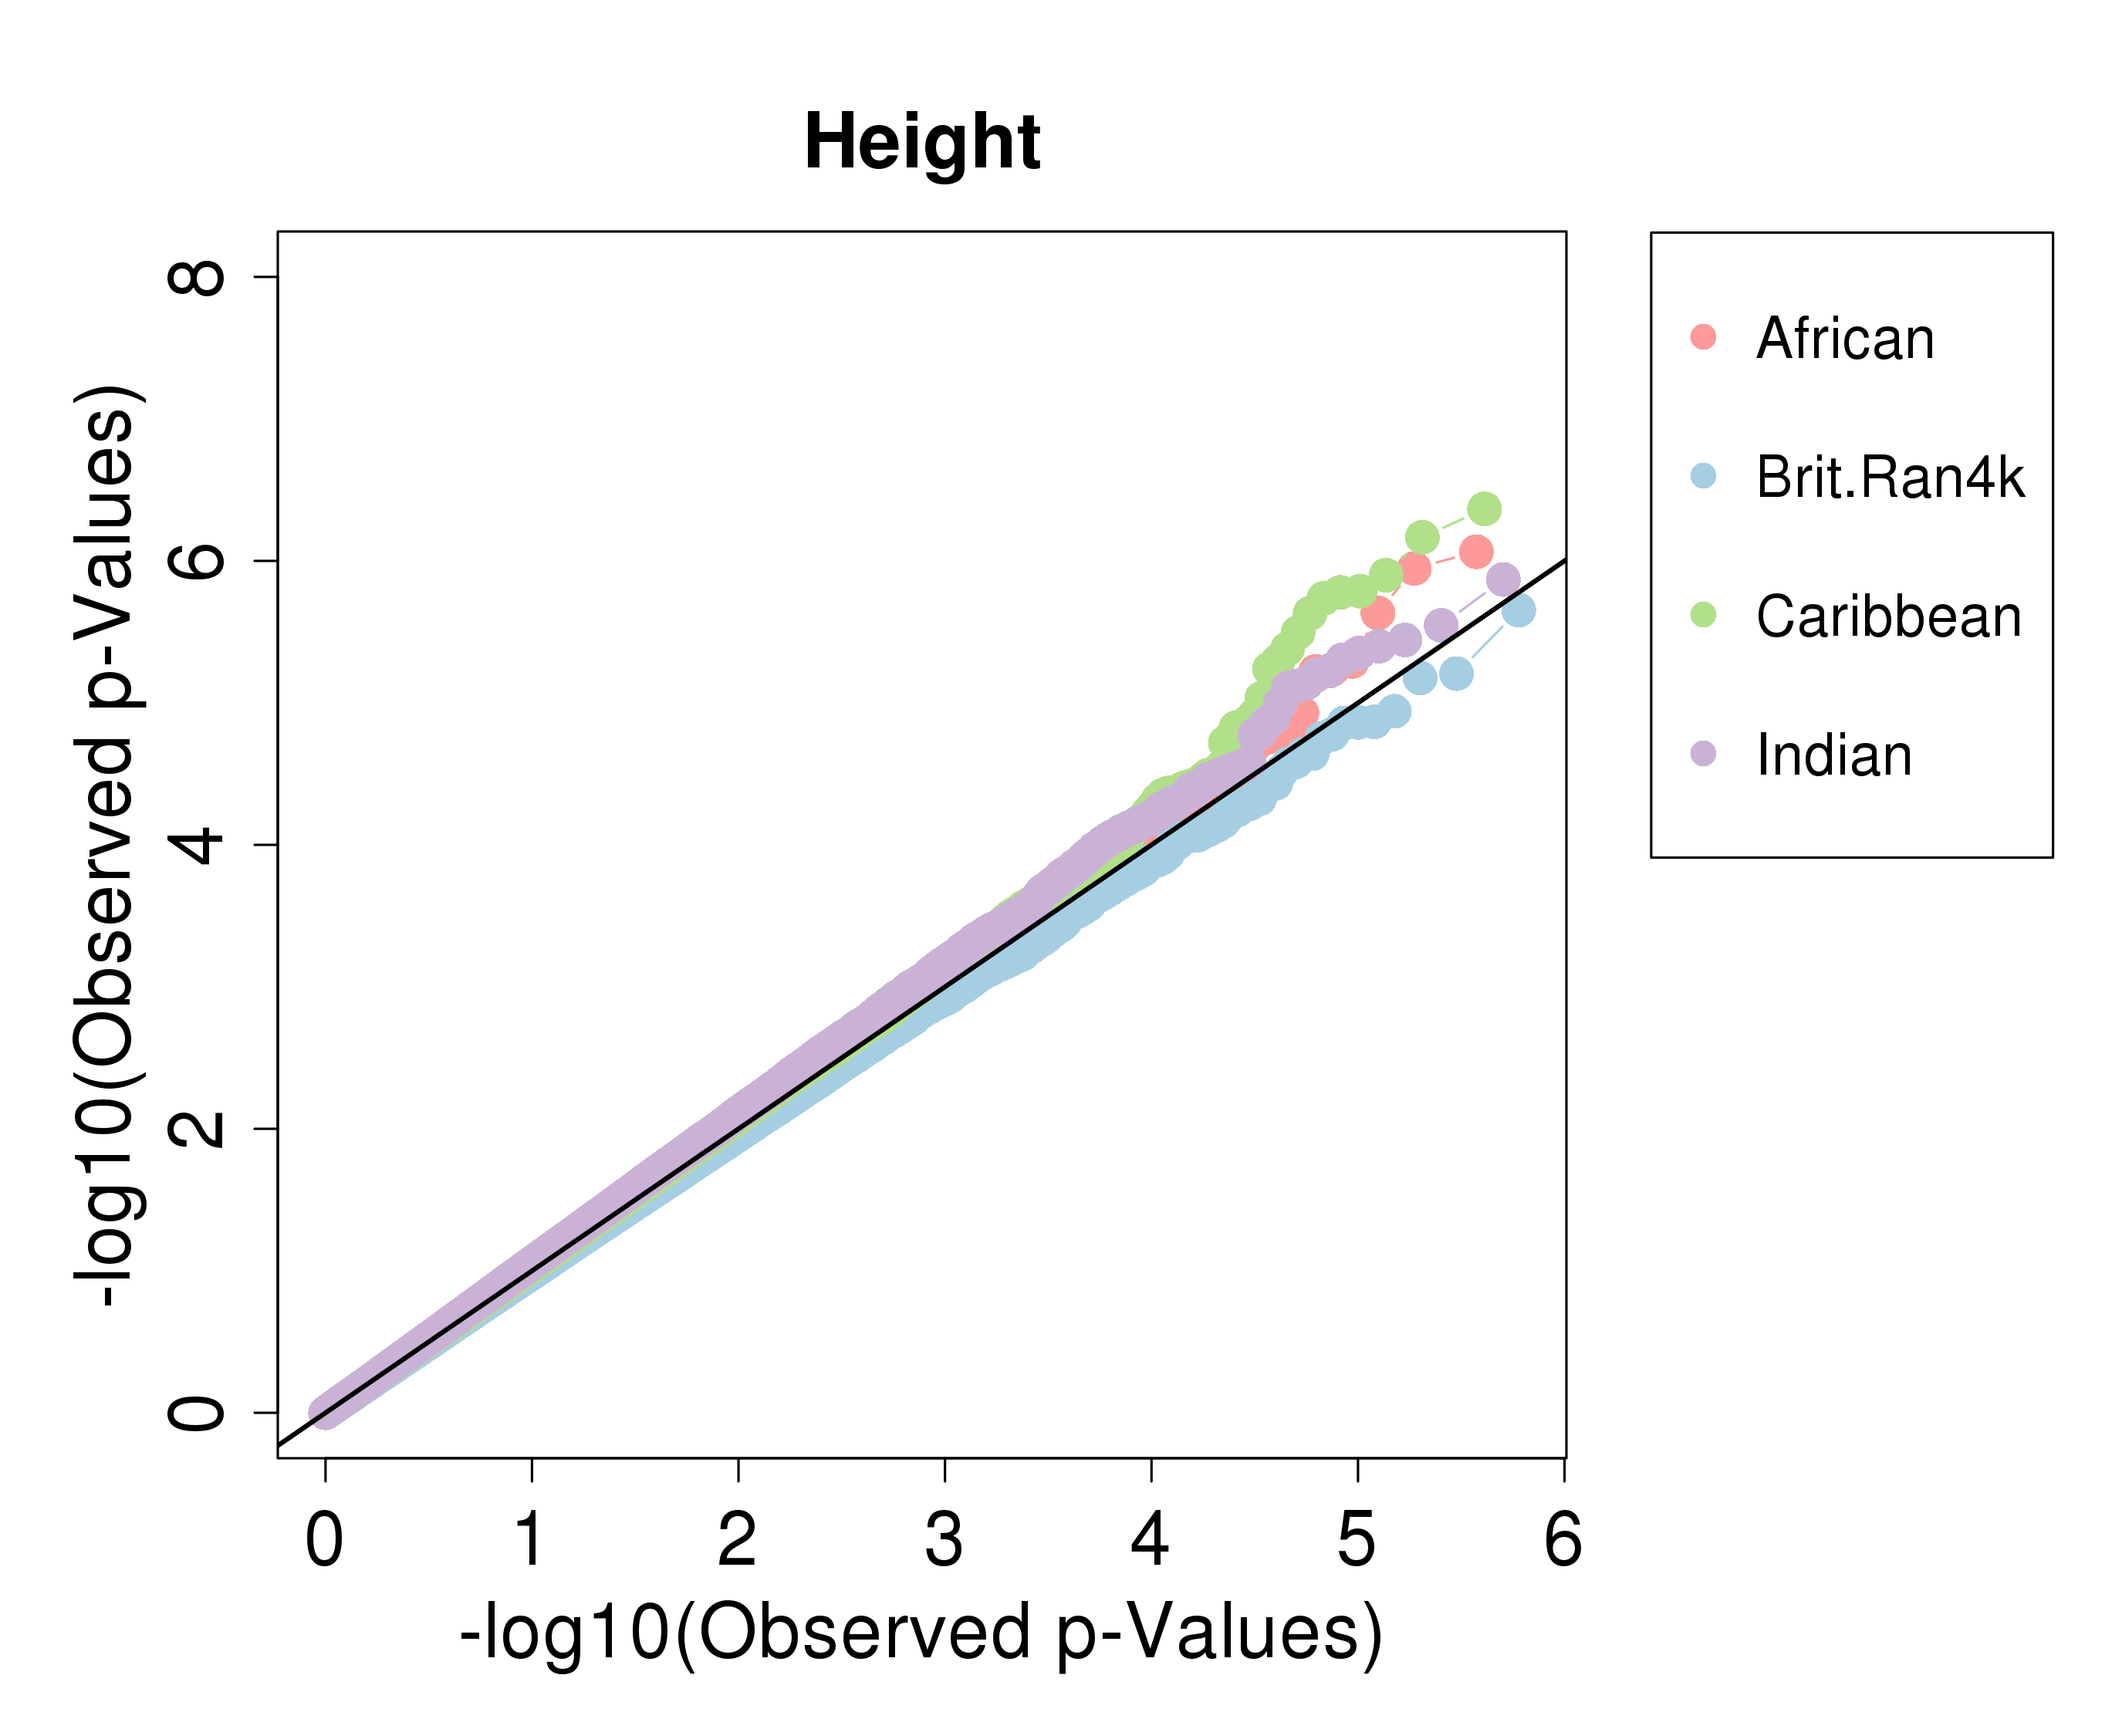
\includegraphics[scale=.35]{Images/Main/InterPath_Main_Figure_MAPIT_vs3_Height.png}
\caption[TBD]{\textbf{MAPIT Results QQ-Plots}. Shown are QQ-plots of our results from running MAPIT on our four initial UKB population subsets in height and BMI. On the $x$-axis are the -$\log_{10}$ of our expected $p$-values and the on the $y$-axis are on the -$\log_{10}$ of our observed $p$-values. We observe weak signals of marginal epistasis across most of the population subsets in height and only a few potential weak signals in BMI. We do observe potential differences across population subsets. However, this lack of signal may be a product of our limited sample sizes, emphasizing the need to increase power through other means, such as by methodological improvements.}
\label{InterPath-Main-Figure-MAPIT-Height}
\end{figure}

There remains the issue though of our limited sample sizes and datasets. While there are ongoing efforts to increase the number of non-European individuals publicly available for complex trait analysis (PAGE,TOPMED refs \cite{}), the number of resources for this pale in comparison to what is available for European individuals. Therefore, we need to identify ways to continue making better use out of the datasets we currently have. One theme that is generally observed for most epistatic analyses, including our first choices here, revolve around the use of single variants. However, it has long been appreciated in other areas, such as additive work, that aggregating evidence for association across multiple variants can increase your power to determine significant results \cite{}. Therefore, we decided to explore whether taking a similar approach for epistatic analyses would lead to a similar increase in power for us here. And the marginal epistasis framework happens to provide a natural jumping off point for just such an extension. 

\subsection{Region-Based Approaches Increase Power To Identify Epistasis}\label{InterPath-Results-PathwayEpistasis}

We expanded the previous MAPIT model into a new framework that goes from looking for marginal epistasis with a single variant to looking for marginal epistasis with an entire biological pathway; we call this approach MAPIT-R, for \underline{MA}rginal e\underline{PI}stasis \underline{T}est of \underline{R}egions. The main change we make to the marginal epistasis model is to go from a single SNP of interest \textbf{k} to a collection of SNPs of interest \textbf{R}. For a full description of this model please see Online Methods, but in brief this change leads to the following, new form of our linear mixed model:

\begin{align}
    & \textbf{y} = \mu + \textbf{R} + \textbf{G} + \textbf{Q} + \boldsymbol{\epsilon} \\
    \textbf{R} \sim \mathcal{MVN}&(\textbf{0}, \phi^{2}\textbf{K}_R) \quad \textbf{G} \sim \mathcal{MVN}(\textbf{0}, \omega^{2}\textbf{K}_G) \nonumber \\ 
    \textbf{Q} \sim \mathcal{MVN}&(\textbf{0}, \sigma^{2}\textbf{K}_Q) \quad \boldsymbol{\epsilon} \sim \mathcal{MVN}(\textbf{0}, \tau^{2}\textbf{I}) \nonumber 
\end{align}
where now R is a new random effects term that represents our new group of SNPs R, with variance component $\phi$ and GRM $\textbf{K}_R$ based on the SNP set R, and where now $\textbf{K}_Q = \textbf{K}_R \circ \textbf{K}_G$, the Hadamard product between the GRMs constructed from R and G. Similar to the MAPIT model, we construct our 'epistasis' random effect by conducting pairwise multiplication, though now it is between two matrices instead of a vector and a matrix. To see how this changes the additive form of the model, see equation XX in Online Methods. We fit this model similarly to before (also see Online Methods), and are interested in whether the variance component term $\sigma$ is significantly greater than 0.

Beyond extending our marginal epistasis model, we also expanded the number of UKB data subsets we analyzed given our encouraging results at the single SNP level. Specifically, we added UKB subsets consisting of Chinese, Pakistani, and Irish ancestry, as well as a second random subset of British individuals representing a larger sample size of close to 10,000 individuals. Both the Irish and new, second British subsets represent large sample size subsets to test how our model performs as sample size increases. Lastly, we chose to analyze the KEGG and REACTOME pathways available from the MSigDB \citep{Liberzon2011} due to their coverage of a wide range of biological processes. 

Running MAPIT-R on our UKB subsets across height and BMI, we find a major increase in our power to detect marginal epistasis. In total across each population subset, phenotype, and pathway database combination, we identified 245 significant genetic interactions between a pathway and the remaining genomic background (Figure \ref{InterPath-Main-Figure-Barplots-KEGGHght}, Supplementary Figure \ref{InterPath-Supp-Figure-Barplots-All}, and Supplementary Tables \ref{InterPath-Supp-Table-TopPathways-KEGG-Height-a}\textcolor{blue}{-d}; $p$-value significance thresholds were determined using Bonferroni multiple testing correction based on the number of pathways tested per analysis). We see both variation in our ability to detect marginal epistasis across our population subsets as well as a much stronger ability to pick up signals in our African subset. Additionally, conducting an analysis run with permuted phenotypes shows that MAPIT-R behaves as expected under the null (Supplementary Figures \ref{InterPath-Supp-Figure-perm1-QQPlots-AllPaths}-\ref{InterPath-Supp-Figure-10perms-pValHists}), and we observe FDR estimates as high as only 1.5\% across our different ancestry, phenotype, and pathway database combinations (Supplementary Table \ref{InterPath-Supp-Tables-AllPops-FDRs}).

\begin{figure}[htbp]
\centering
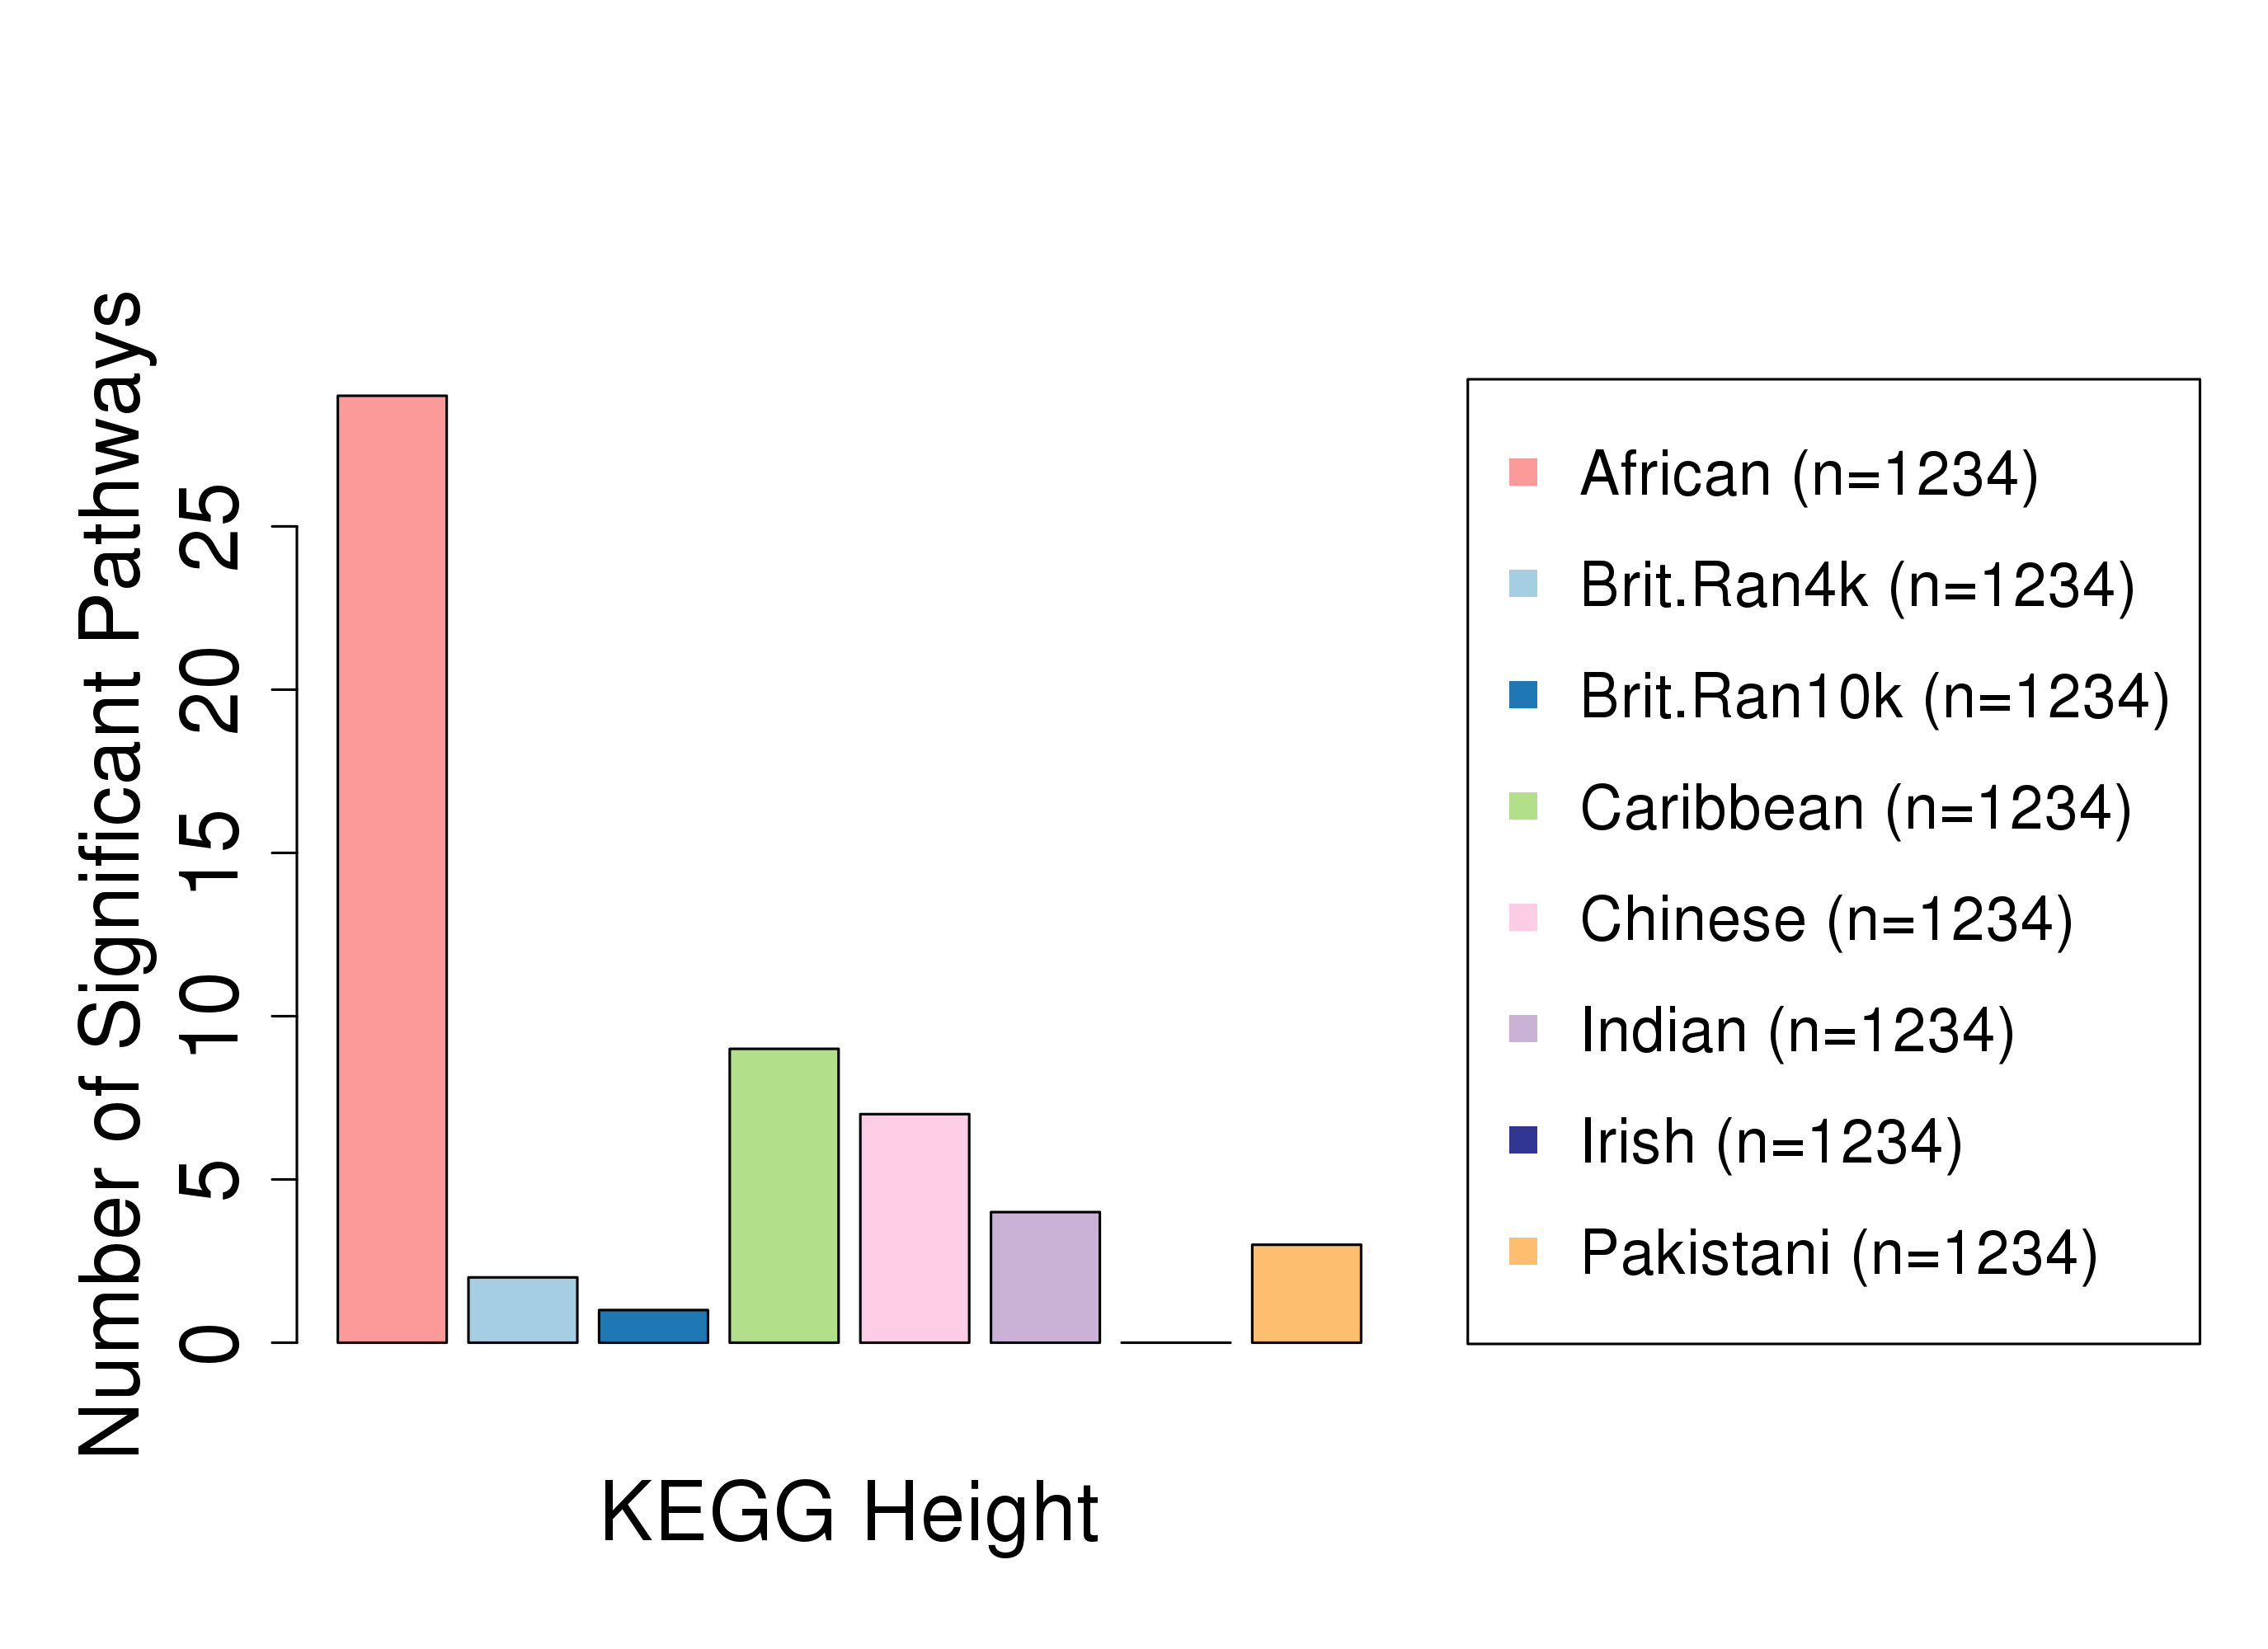
\includegraphics[scale=.35]{Images/Main/InterPath_Main_Figure_Barplots_KEGGHght_vs1.png}
\caption[TBD]{\textbf{Number of Significant Pathways from Running MAPIT-R on UKB subsets}. Shown are the number of significant pathways found from running MAPIT-R on each of our expanded collection of UKB population subsets using height and BMI in the KEGG database (REACTOME results can be found in Supplementary Figure XX). A pathway is considered significant if its MAPIT-R $p$-value is below XXX (.05 / XXX, the number of KEGG pathways tested). We find that the African population far and away has the largest number of significant pathways, both for each phenotype and for each pathway database. But in general we also tend to see significant pathways moreso in non-European populations than European populations.}
\label{InterPath-Main-Figure-Barplots-KEGGHght}
\end{figure}

In fact the vast majority of our significant interactions are represented in the African subset (165/245). This stands out because the African subset is neither our population with the largest sample size or our population with the largest number of SNPs. We do see a significant relationship between number of SNPs in a pathway and that pathway's MAPIT-R $p$-value (Supplementary Figure \ref{InterPath-Supp-Figure-pValsVsNumSNPs}), however the African subset has similar pathway SNP counts amongst its top pathways as compared to the other population subsets. One possibility for this result may be an ascertainment bias from using variants based on a genotyping chip that was developed primarily using European data. Simulations that replicate such an ascertainment bias however show no evidence of this leading to an increase in power (Supplementary Figure XX). Additionally, it is unlikely that our results are produced from excess cryptic population structure as well; simulations that specifically model different population structure schemes show no evidence for a bias in our results (Supplementary Figure XX \textcolor{red}{(this is where the proposed simulation results would go)}). 


\subsection{Beginning Examples of Ancestry-Level Differences in Epistatic Interactions}

Looking at the specific pathways that we observe as having significant evidence for marginal epistasis, it does not appear that we can confidently infer population-specific examples of pathway marginal epistasis. Most genome-wide significant pathways in any non-African subset overlap with a genome-wide significant pathway in the African subset (Figure \ref{InterPath-Main-Figure-Heatplots-KEGG} \& Supplementary Figure \ref{InterPath-Supp-Figure-Heatplots-AllPaths}). Interestingly, while we do witness that while most populations overlap with the African subset, there is often little overlap among the non-African subsets; for example in KEGG BMI the Caribbean subset overlaps with African for 6 of its 7 pathways, and the Chinese subset overlaps with the African subset for 7 of its 8 pathways, but there is no overlap between the Chinese and Caribbean subsets.

\begin{figure}[htbp]
\centering
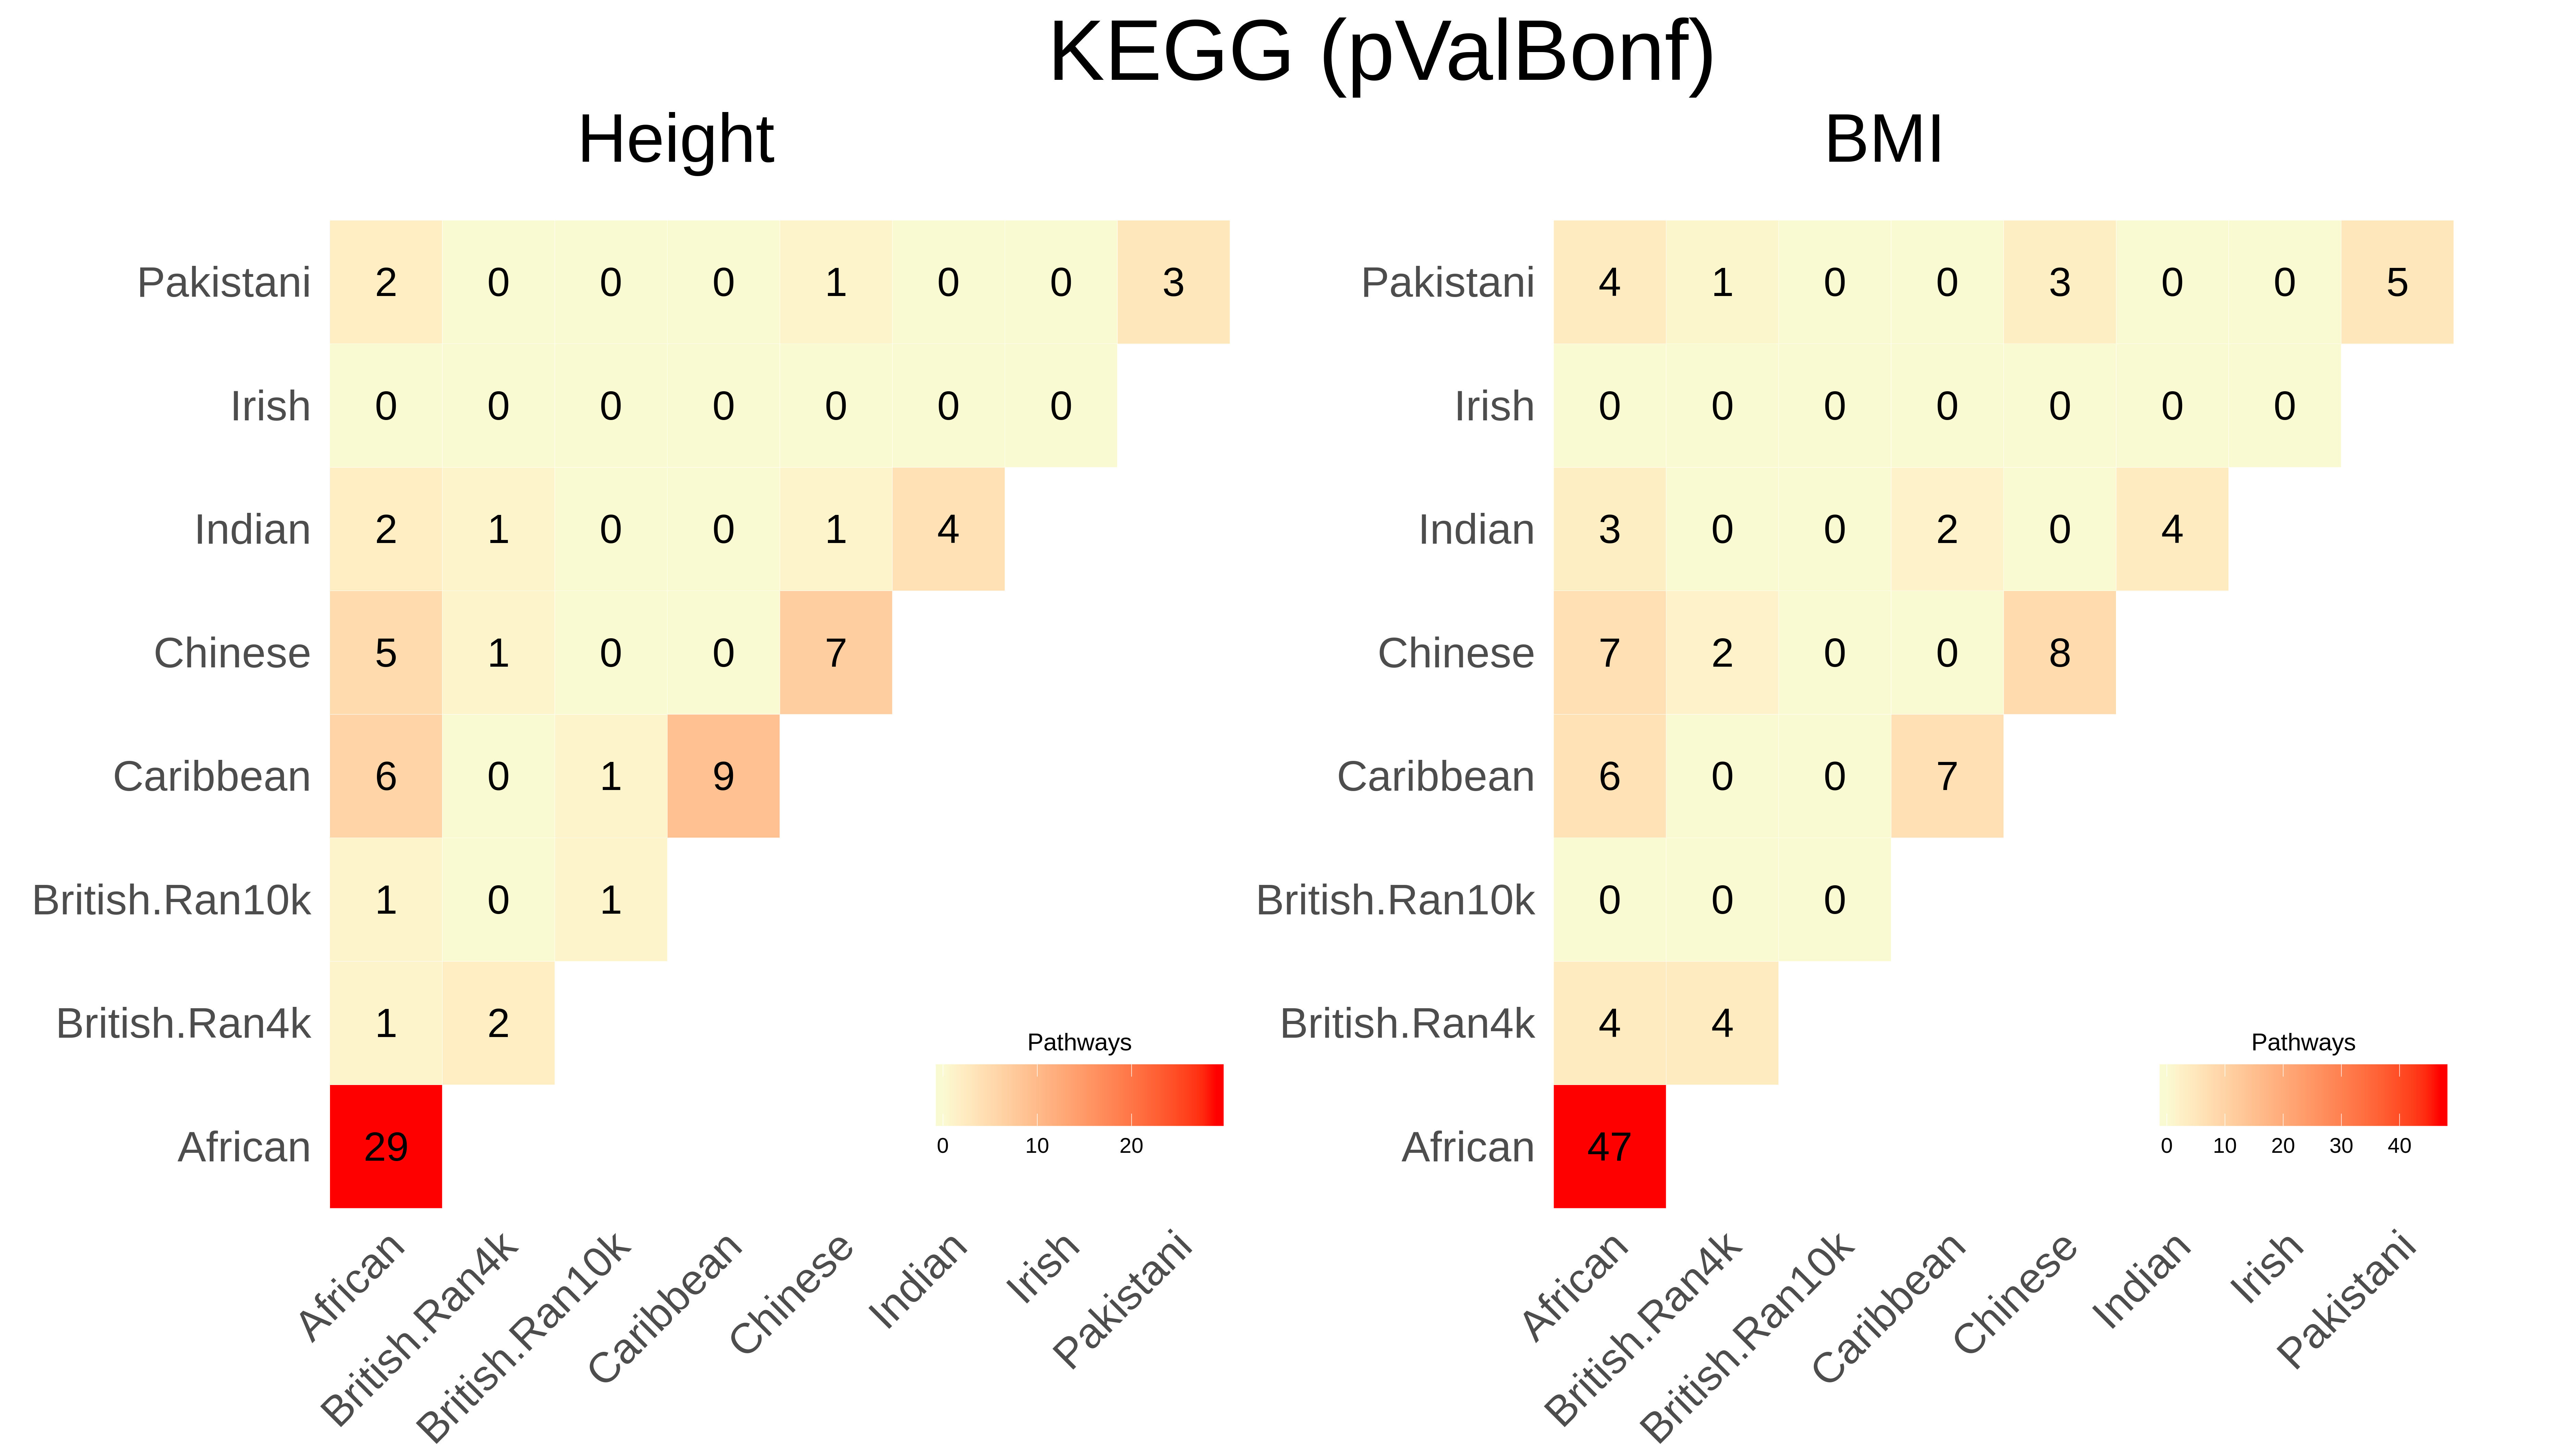
\includegraphics[scale=.225]{Images/Main/InterPath_Main_Figure_Heatplots_KEGG_vs1.png}
\caption[TBD]{\textbf{Overlap of Significant MAPIT-R Pathways Between UKB Population Subsets}. \\ Shown are the numbers of significant MAPIT-R pathways that overlap between each populations for both height and BMI in the KEGG database. A pathway is considered significant as defined in Figure \ref{InterPath-Main-Figure-Barplots}. The diagonal (overlap between the same populations) shows the total number of significant pathways per population subset. As observed in Figure \ref{InterPath-Main-Figure-Barplots}, we find that the African subset has a much larger number of significant pathways than any other population subset. We also observe that most of the significant pathways in other populations overlap with the significant pathways seen in the African subset. These top KEGG pathways can be seen in Supplementary Table \ref{InterPath-Supp-Table-TopPathways-KEGG-Height-a}.}
\label{InterPath-Main-Figure-Heatplots-KEGG}
\end{figure}

\subsection{The Proteasome as a Candidate Protein Complex Enriched for Epistatic Interactions}

As previously mentioned, we observe that genome-wide significant pathways across subsets tend to be the pathways with the largest numbers of SNPs. While this is not surprising given that these are the pathways which potentially have the most power to identify a positive signal, we only have a limited number of these types of pathways to compare against one another; it is unclear if these particular pathways represent interesting biology specific to our complex traits or are moreso indicative of there being widespread, but indiscriminate, epistasis across the genome. One approach to decouple significant pathways from having a large number of SNPs is to simply look at the collection of top pathways with the least number of SNPs. For example, we observe 26 number of pathways in the African BMI REACTOME analysis that included less than 1000 SNPs. To identify whether there are common biological underpinnings across these pathways, we first looked at whether any groups of genes were enriched across these pathways. And indeed, we observe for many genes that are highly represented across these pathways, that they are significantly enriched (Supplementary Tables \ref{InterPath-Supp-Tables-AllPops-TopGeneCounts-KEGG-Height-a}\textcolor{blue}{-d}).

However, the hypergeometric test that underlies these enrichment results assumes independence between pathways, and we know that to not be the case. To get a better sense of what our expectations for the results should be, we instead reran these analyses using the full set of significant pathways, not just those with SNP counts below 1000. Our hypothesis is that if the full set of results are confounded by some pathways just having many more SNPs than real biological signals, the noise-to-signal ratio should get worse for the genes that represented true biology. And indeed when we rerun this analysis, we observe for a specific group of genes, those related to the proteasome complex, that their enrichment $p$-values become less significant going from the more refined set of smaller significant pathways to the more general set of total significant pathways (Supplementary Table \ref{InterPath-Supp-Tables-AllPops-TopGeneCount-HypergeometricTests}. These gene families (PSMA*, PSMB*, PSMC*, PSMD*, and PSME*) represent different subunits of the proteasome complex, a catalytic protein structure that is essential to the ubiquitination degradation pathway. Interestingly, the proteasome may be a reasonable candidate for having biologically important genetic interactions with the rest of the genome -- it is likely to be involved with a large number of distinct biological processes, though always in the same capacity. It is possibly unsurprising then that we find this gene enrichment in BMI and not height, since metabolism inherently involves the degradation of molecules. 

%To further look into these proteasome genes, we...

\subsection{Testing the Null Model with British Replicate Subpopulations}

One important consideration of our results is that we have limited representations of the different human ancestries we are analyzing. Are the samples we are analyzing large enough to be representative of the true total populations? While it is still difficult to address that question directly for non-European populations due to the limited availability of other public datasets, we are able to ask that question for the British ancestry subsets. Specifically, we can take additional, non-overlapping random subsets of 4,000 and 10,000 British individuals and see if they are at least consistent in their lack of results as compared to each original random subset. And indeed this is what we observe when we take an additional 4 random subsets of British individuals at each sample size: similar low numbers of significant pathways, very little overlap in significant pathways across replicates, and similar behavior under the null (Supplementary Figures \ref{InterPath-Supp-Figure-BritReps-Barplots}-\ref{InterPath-Supp-Figure-BritReps-10perms-pValHists-pt1} and Supplementary Table \ref{InterPath-Supp-Tables-BritReps-FDRs-pt1}). This at least indicates that we are unlikely to observe the large levels of significant results we witness in the African subset by simply choosing a 'better' collection of individuals by chance.  

\subsection{Investigating the Relationship Between Within-Population Genetic Variation and Detecting Epistasis}

One of the clearest results from the MAPIT-R analyses is that the African subset has much greater levels of evidence for pathway marginal epistasis than any other UKB subset. An obvious next question then is why. One of the most well-appreciated genetic architecture patterns in African populations versus other global human populations is the much greater levels of genetic diversity found in African versus out-of-African populations. This alignment of patterns then may be a good starting point, especially since greater levels of genetic variation in the underlying data may increase our power to detect epistasis, as suggested by our previous result of more SNPs being positive correlated with more significant MAPIT-R $p$-values. 

Our first approach to investigate this question then was to look at broadscale metrics of genetic variation across our population subsets. We did this by calculating both pairwise Fst values between each subset as well as PVE estimates for each subset's top 10 local principal component (Figures \ref{InterPath-Main-Figure-Fst} \& \ref{InterPath-Main-Figure-Eigenvalues}). For pairwise Fst, we find values get as large as .124, which seem to be within range of previous global sample estimates \cite{Wang2012}. We find that while the African subset does have some of the largest divergences from other populations (such as the British subsets), we also witness close to similar levels of divergence between the Chinese subset and other populations as well. In contract, looking at the top local PC PVE estimates, we see a pattern of population differentiation that is more similar to our MAPIT-R results. The African subset has a PC1 PVE that is much greater than any other population, and the second highest population is the Caribbean cohort, which is also the population with the second most significant MAPIT-R results. We do witness however higher baseline levels of PVE across the other population subsets as compared to the African and Caribbean ones. These results might suggest that what is driving our MAPIT-R results is not solely high levels of genetic variation or differentiation, but also a quality of how this variation is structured within a given population as well.

\begin{figure}[htbp]
\centering
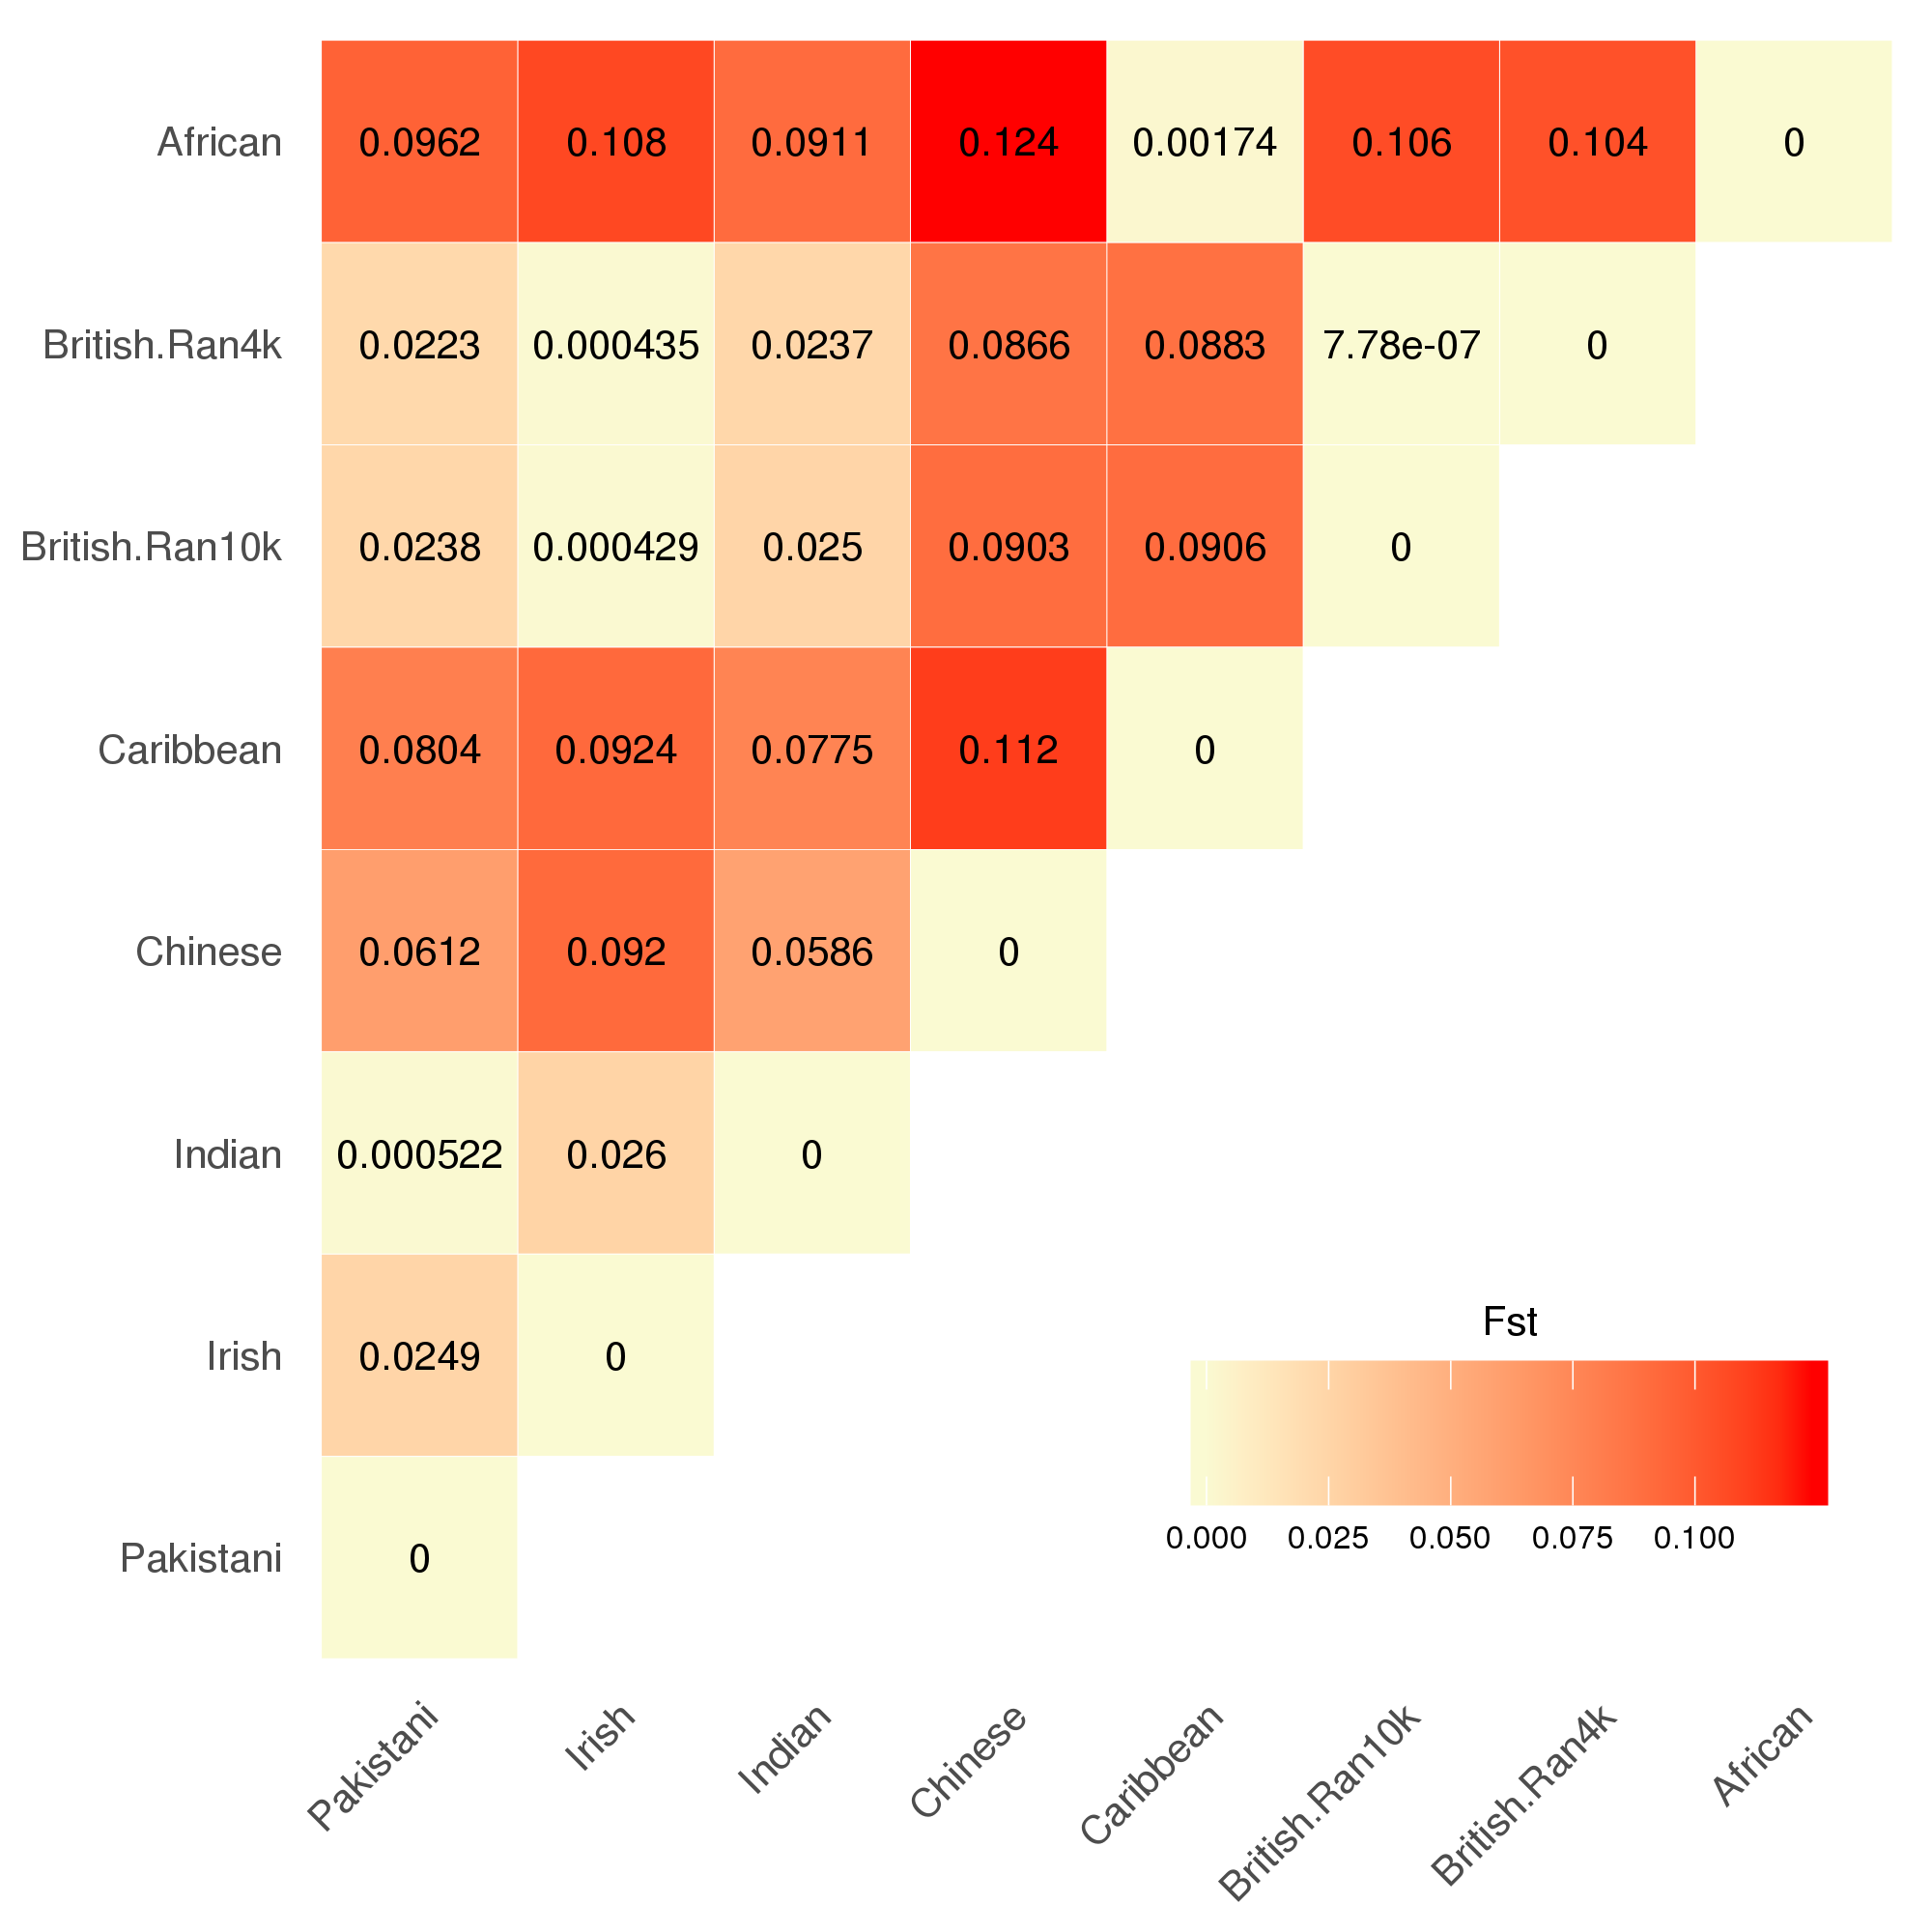
\includegraphics[scale=.5]{Images/Main/InterPath_Main_Figure_Fst_vs1.png}
\caption[TBD]{\textbf{UKB Population Subsets Pairwise Fst} . }
\label{InterPath-Main-Figure-Fst}
\end{figure}

\begin{figure}[htbp]
\centering
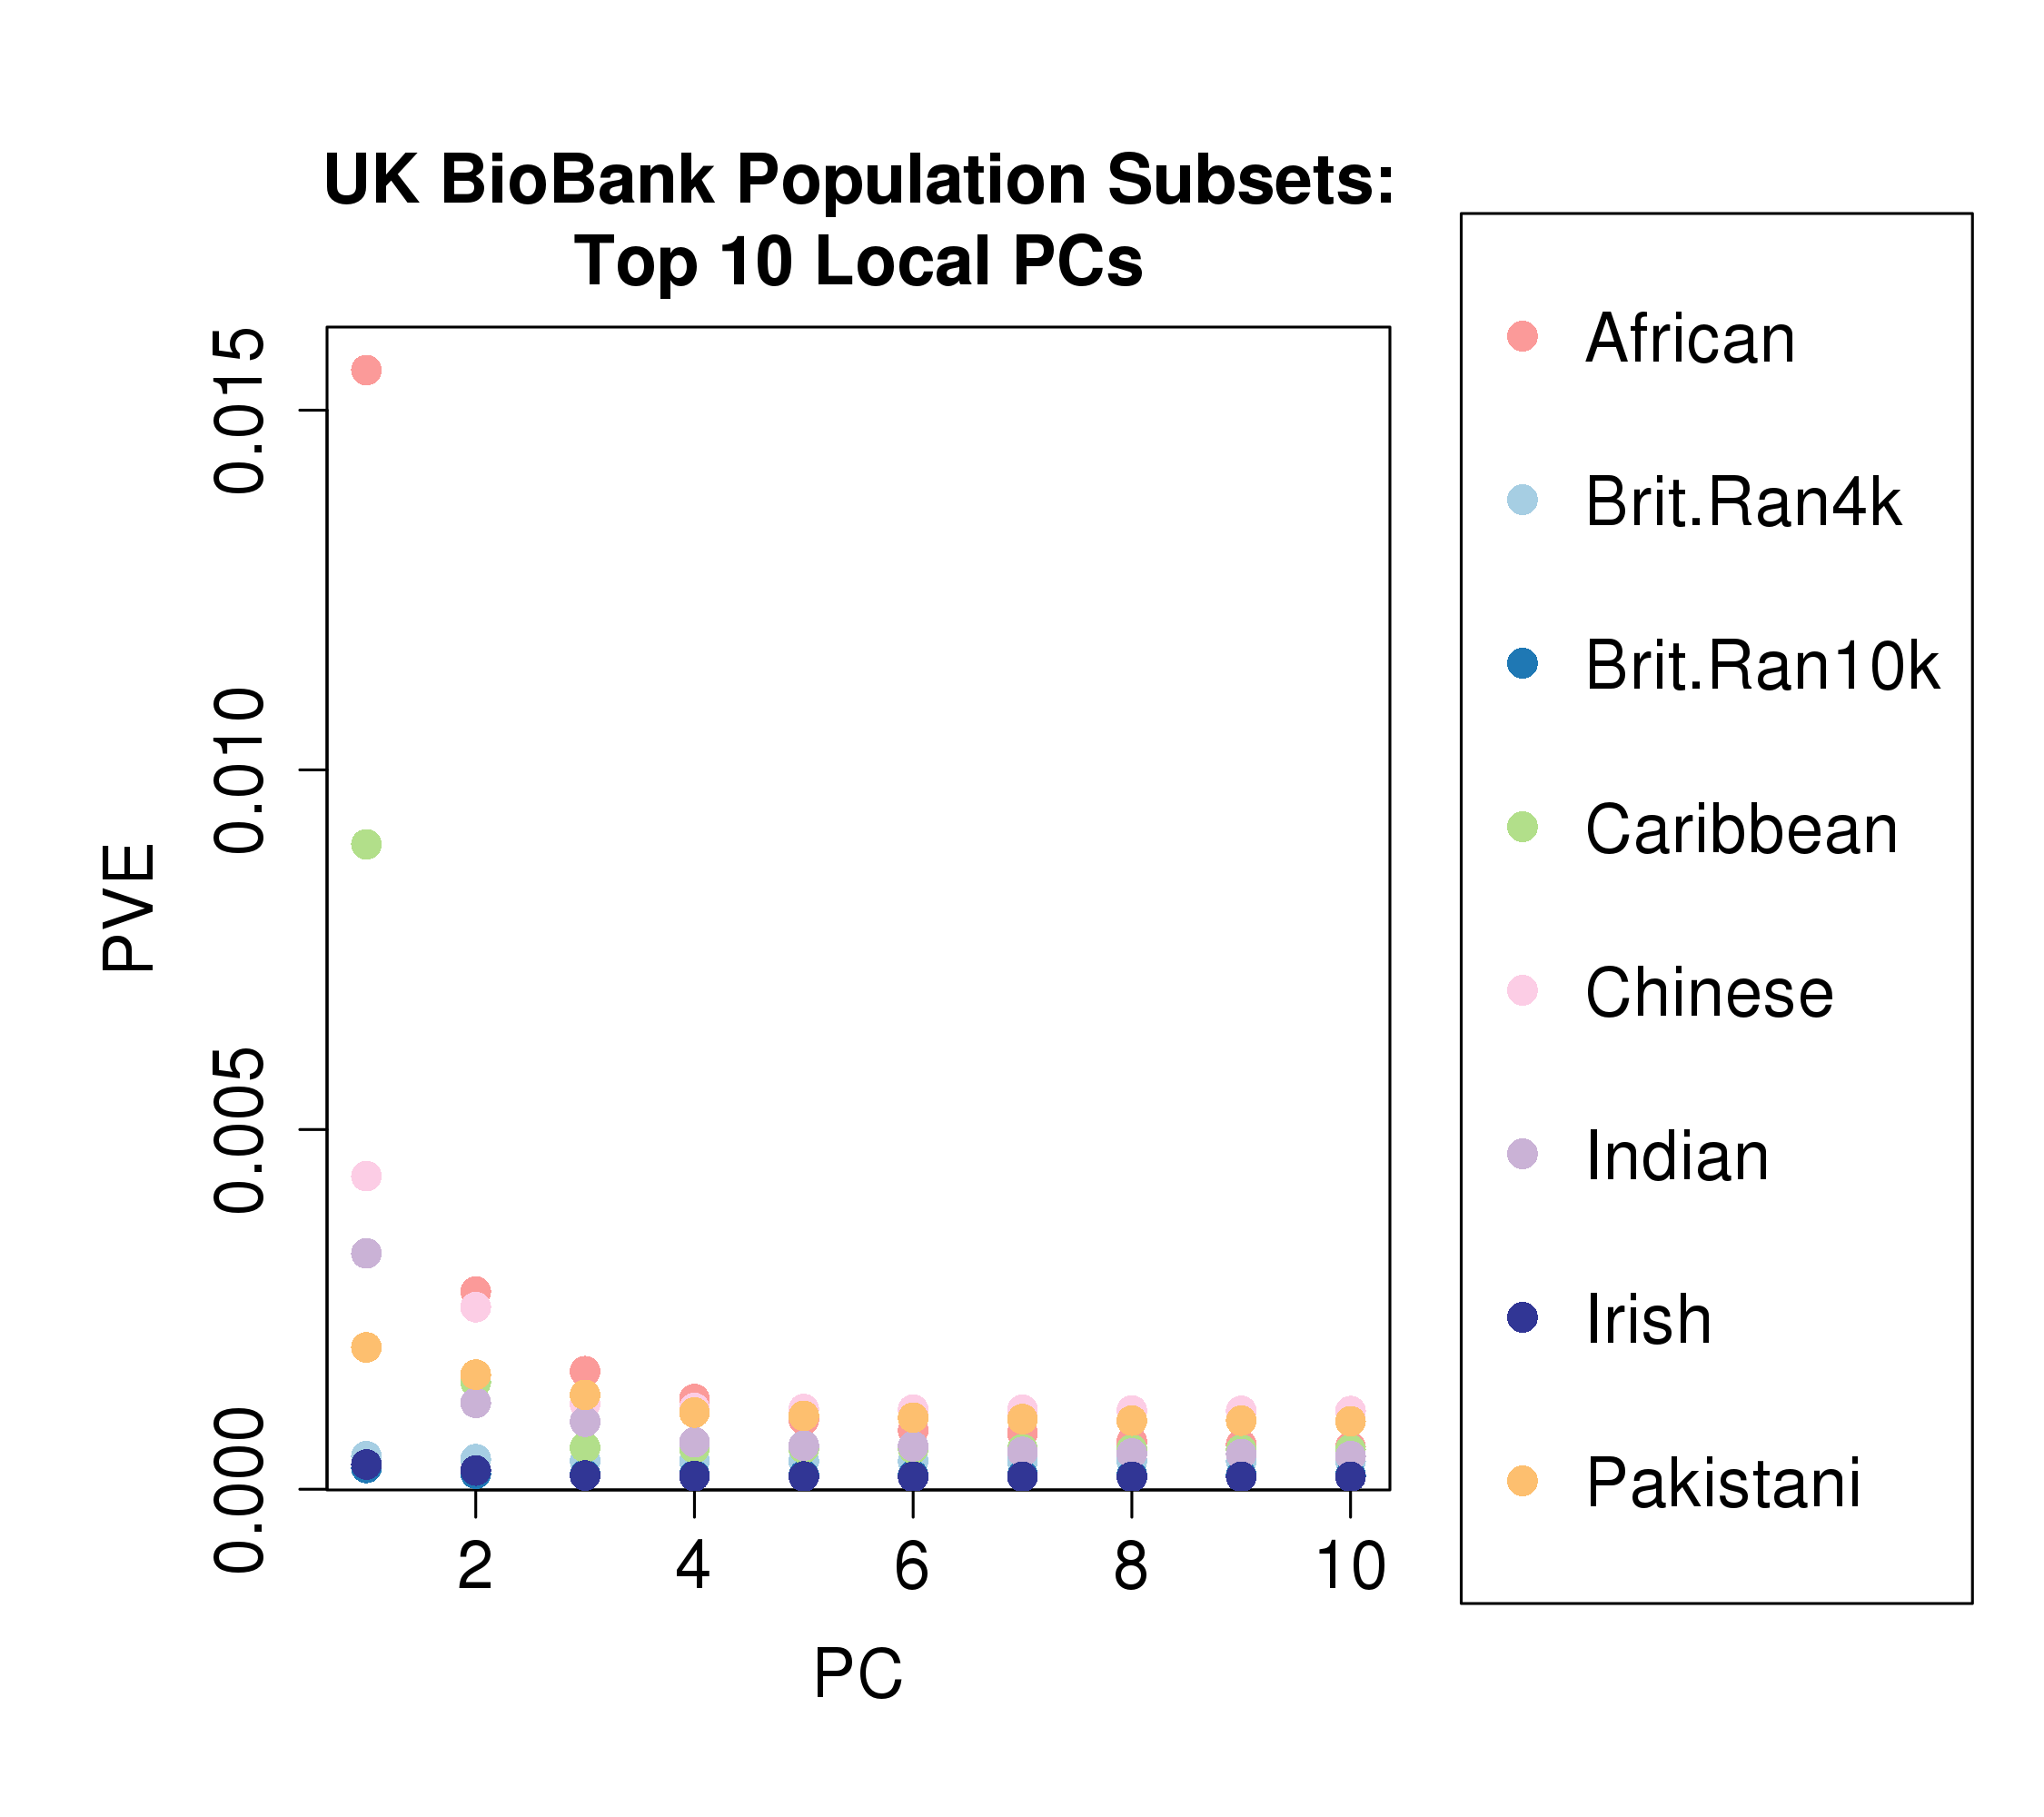
\includegraphics[scale=.5]{Images/Main/InterPath_Main_Figure_Eigenvalues_vs1.png}
\caption[TBD]{\textbf{UKB Population Subsets Top 10 PC Eigenvalues}.}
\label{InterPath-Main-Figure-Eigenvalues}
\end{figure}

To take these analyses one step further, we tried to investigate levels of genetic diversity on the pathway-scale to see if they match up with the observed MAPIT-R results. To accomplish this, we calculated the mean proportion of pairwise identity-by-state across every pair of individuals using all the genotypes of a given pathway. Meaning for a single pathway, we had a metric ranging from 0 to 1 where 1 indicates all pairs of individuals had exactly the same genotypes at every SNP for a given pathway and 0 means all pairs of individuals had completely different genotypes at each of these SNPs. Lower values would then indicate greater levels of genetic diversity for a given a pathway within that ancestry subset. Once we had these values, we then compared them against each pathway's MAPIT-R $p$-value; interestingly, we found there was no relationship between these two metrics (Figure \ref{InterPath-Main-Figure-IBS-AfrHght} \& Supplementary Figure \ref{InterPath-Supp-Figure-IBS-AllPops}). This was true across almost every one of our UKB population subsets, phenotype, and pathway database collections. And in general it does not appear that this lack of relationship changes much per-ancestry either; directly comparing population subsets against one another shows that the per-pathway IBS proportions follow similar trajectories, shifted only by each population's mean level of IBS (Figure \ref{InterPath-Main-Figure-IBS-AllPopComps-AfrHght} \& Supplementary Figure \ref{InterPath-Supp-Figure-IBS-AllPopComps}). Therefore it appears this further supports our previous finding that the signal we are observing in our results is likely not being driven by broadscale levels of genetic variation. There is a more cryptic structure and relationship between the genetic variation in each subset and the epistasis we are observing with MAPIT-R. 

\begin{figure}[htbp]
\centering
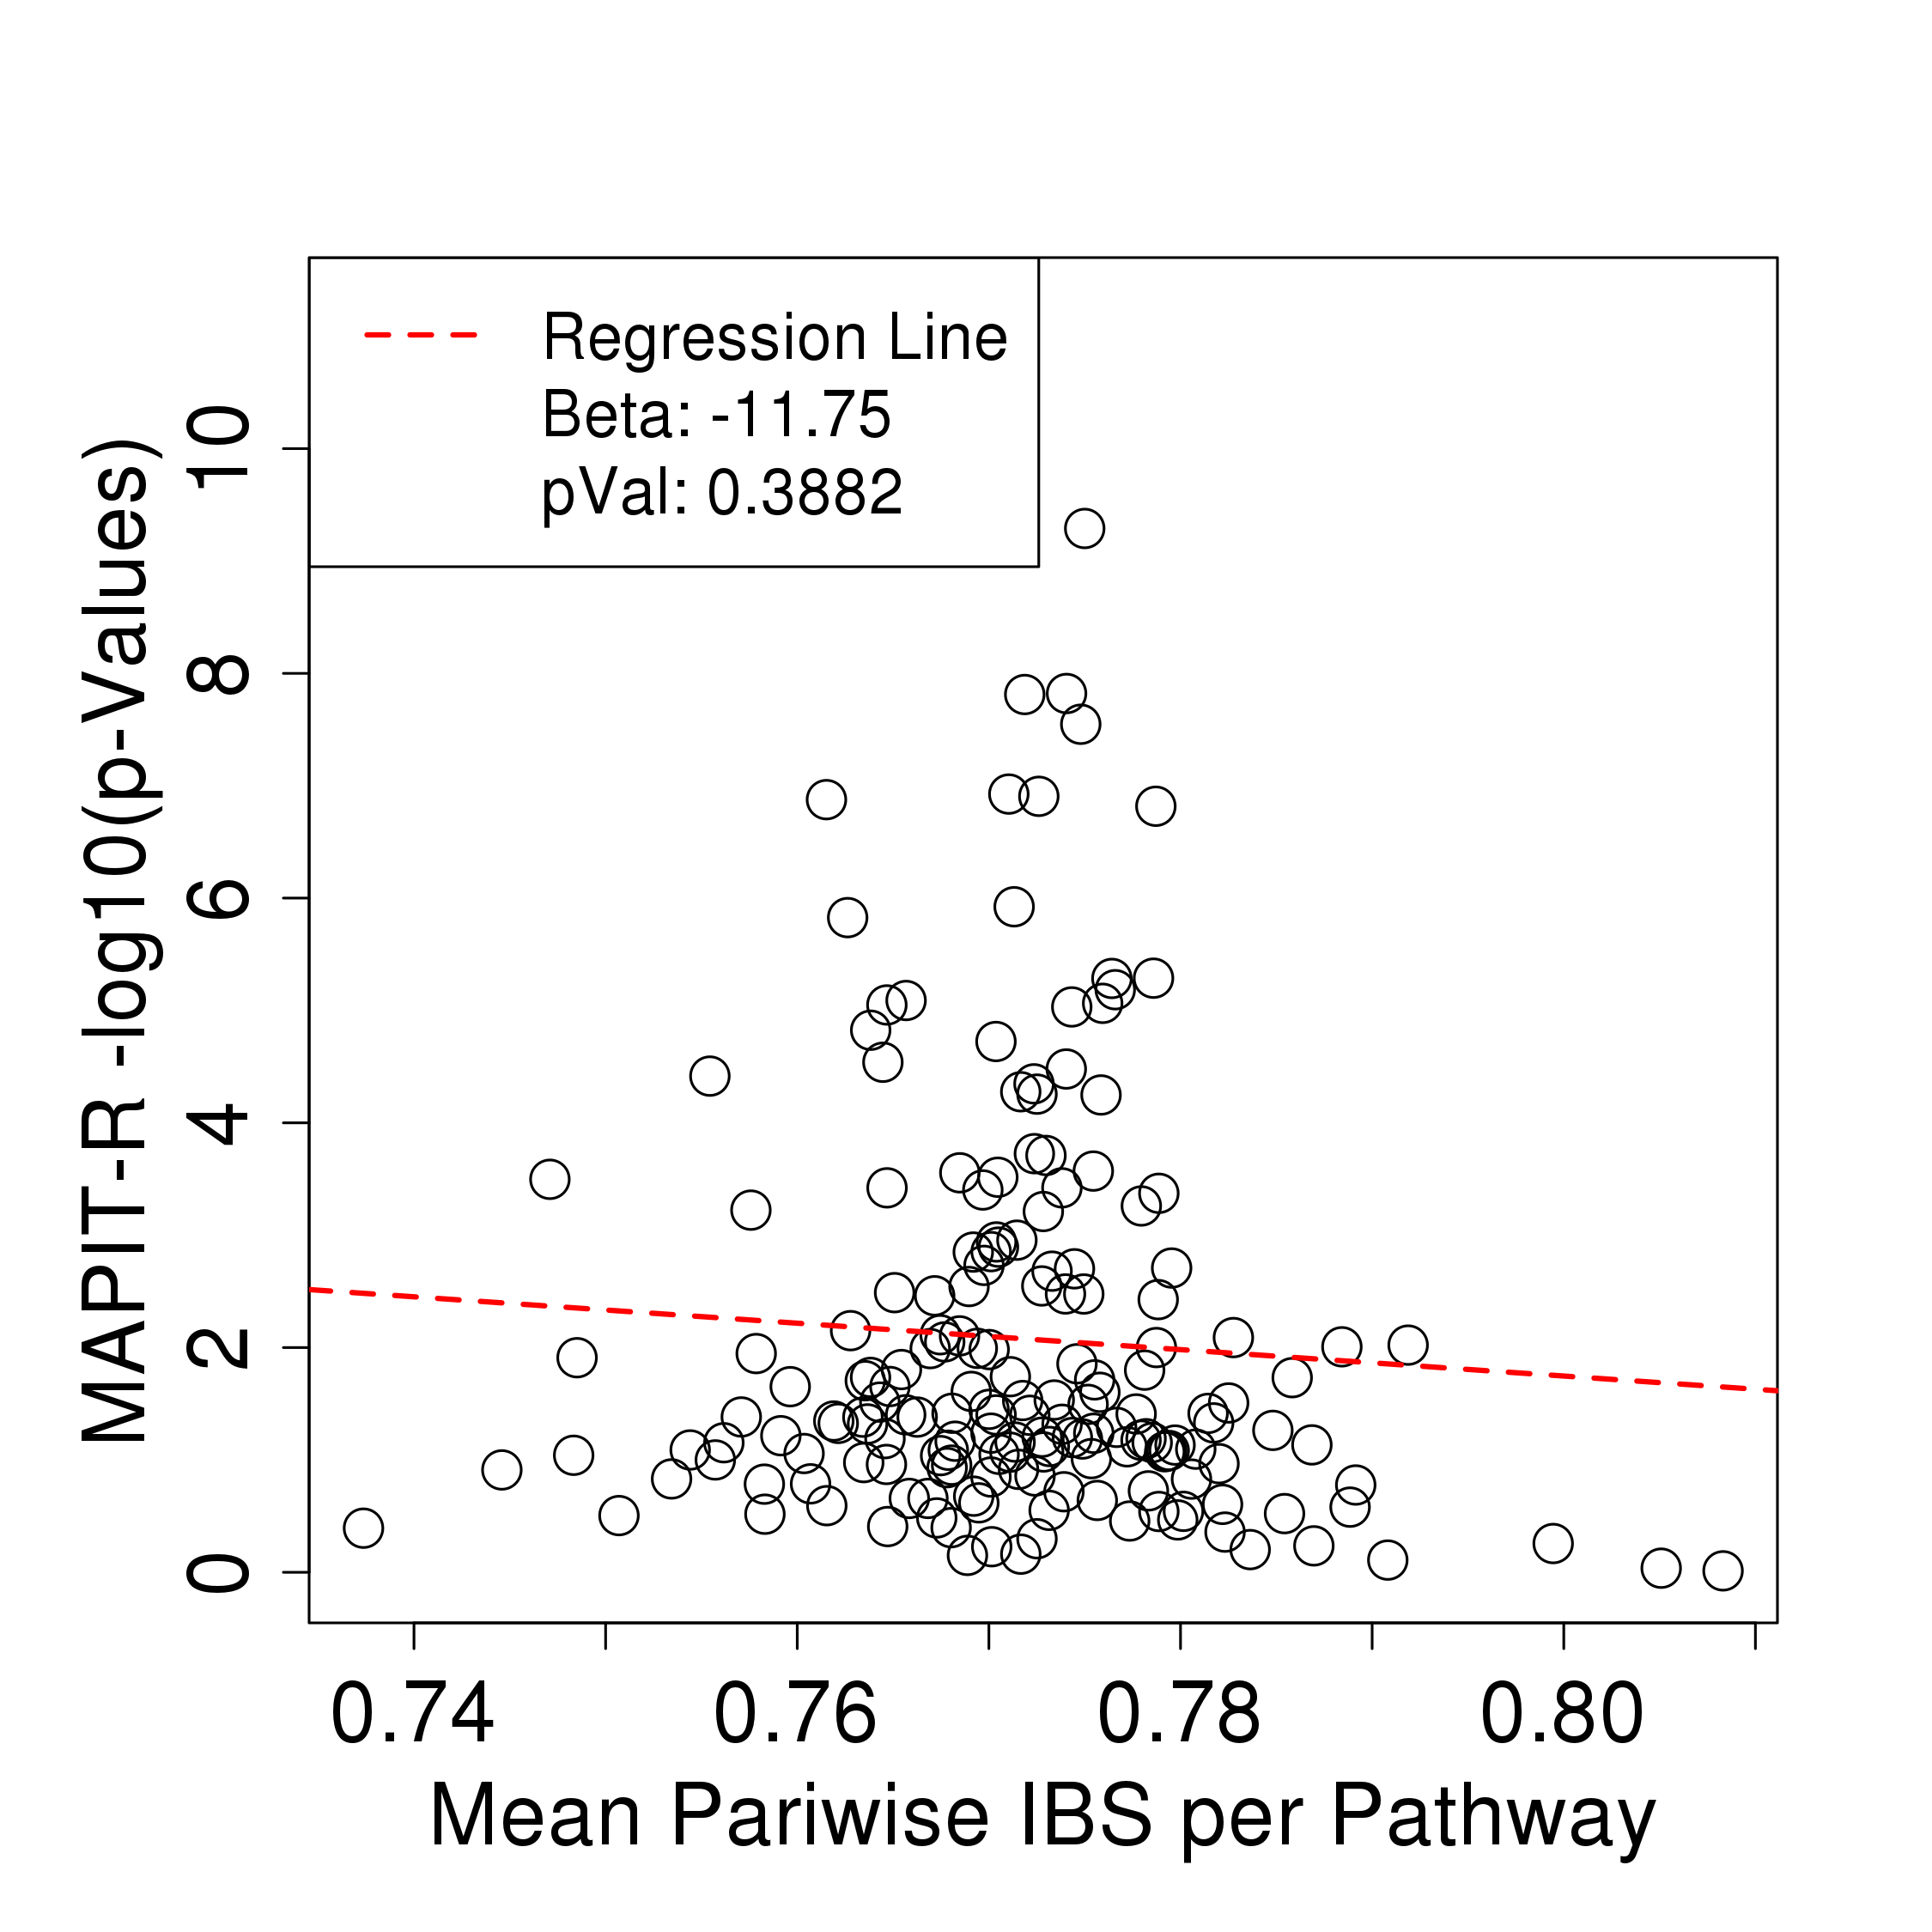
\includegraphics[scale=.35]{Images/Main/InterPath_Main_Figure_IBS_vs2_AfrHght.png}
\caption[TBD]{\textbf{IBS Proportions vs. MAPIT-R $p$-values in African Subset}}
\label{InterPath-Main-Figure-IBS-AfrHght}
\end{figure}

\begin{figure}[htbp]
\centering
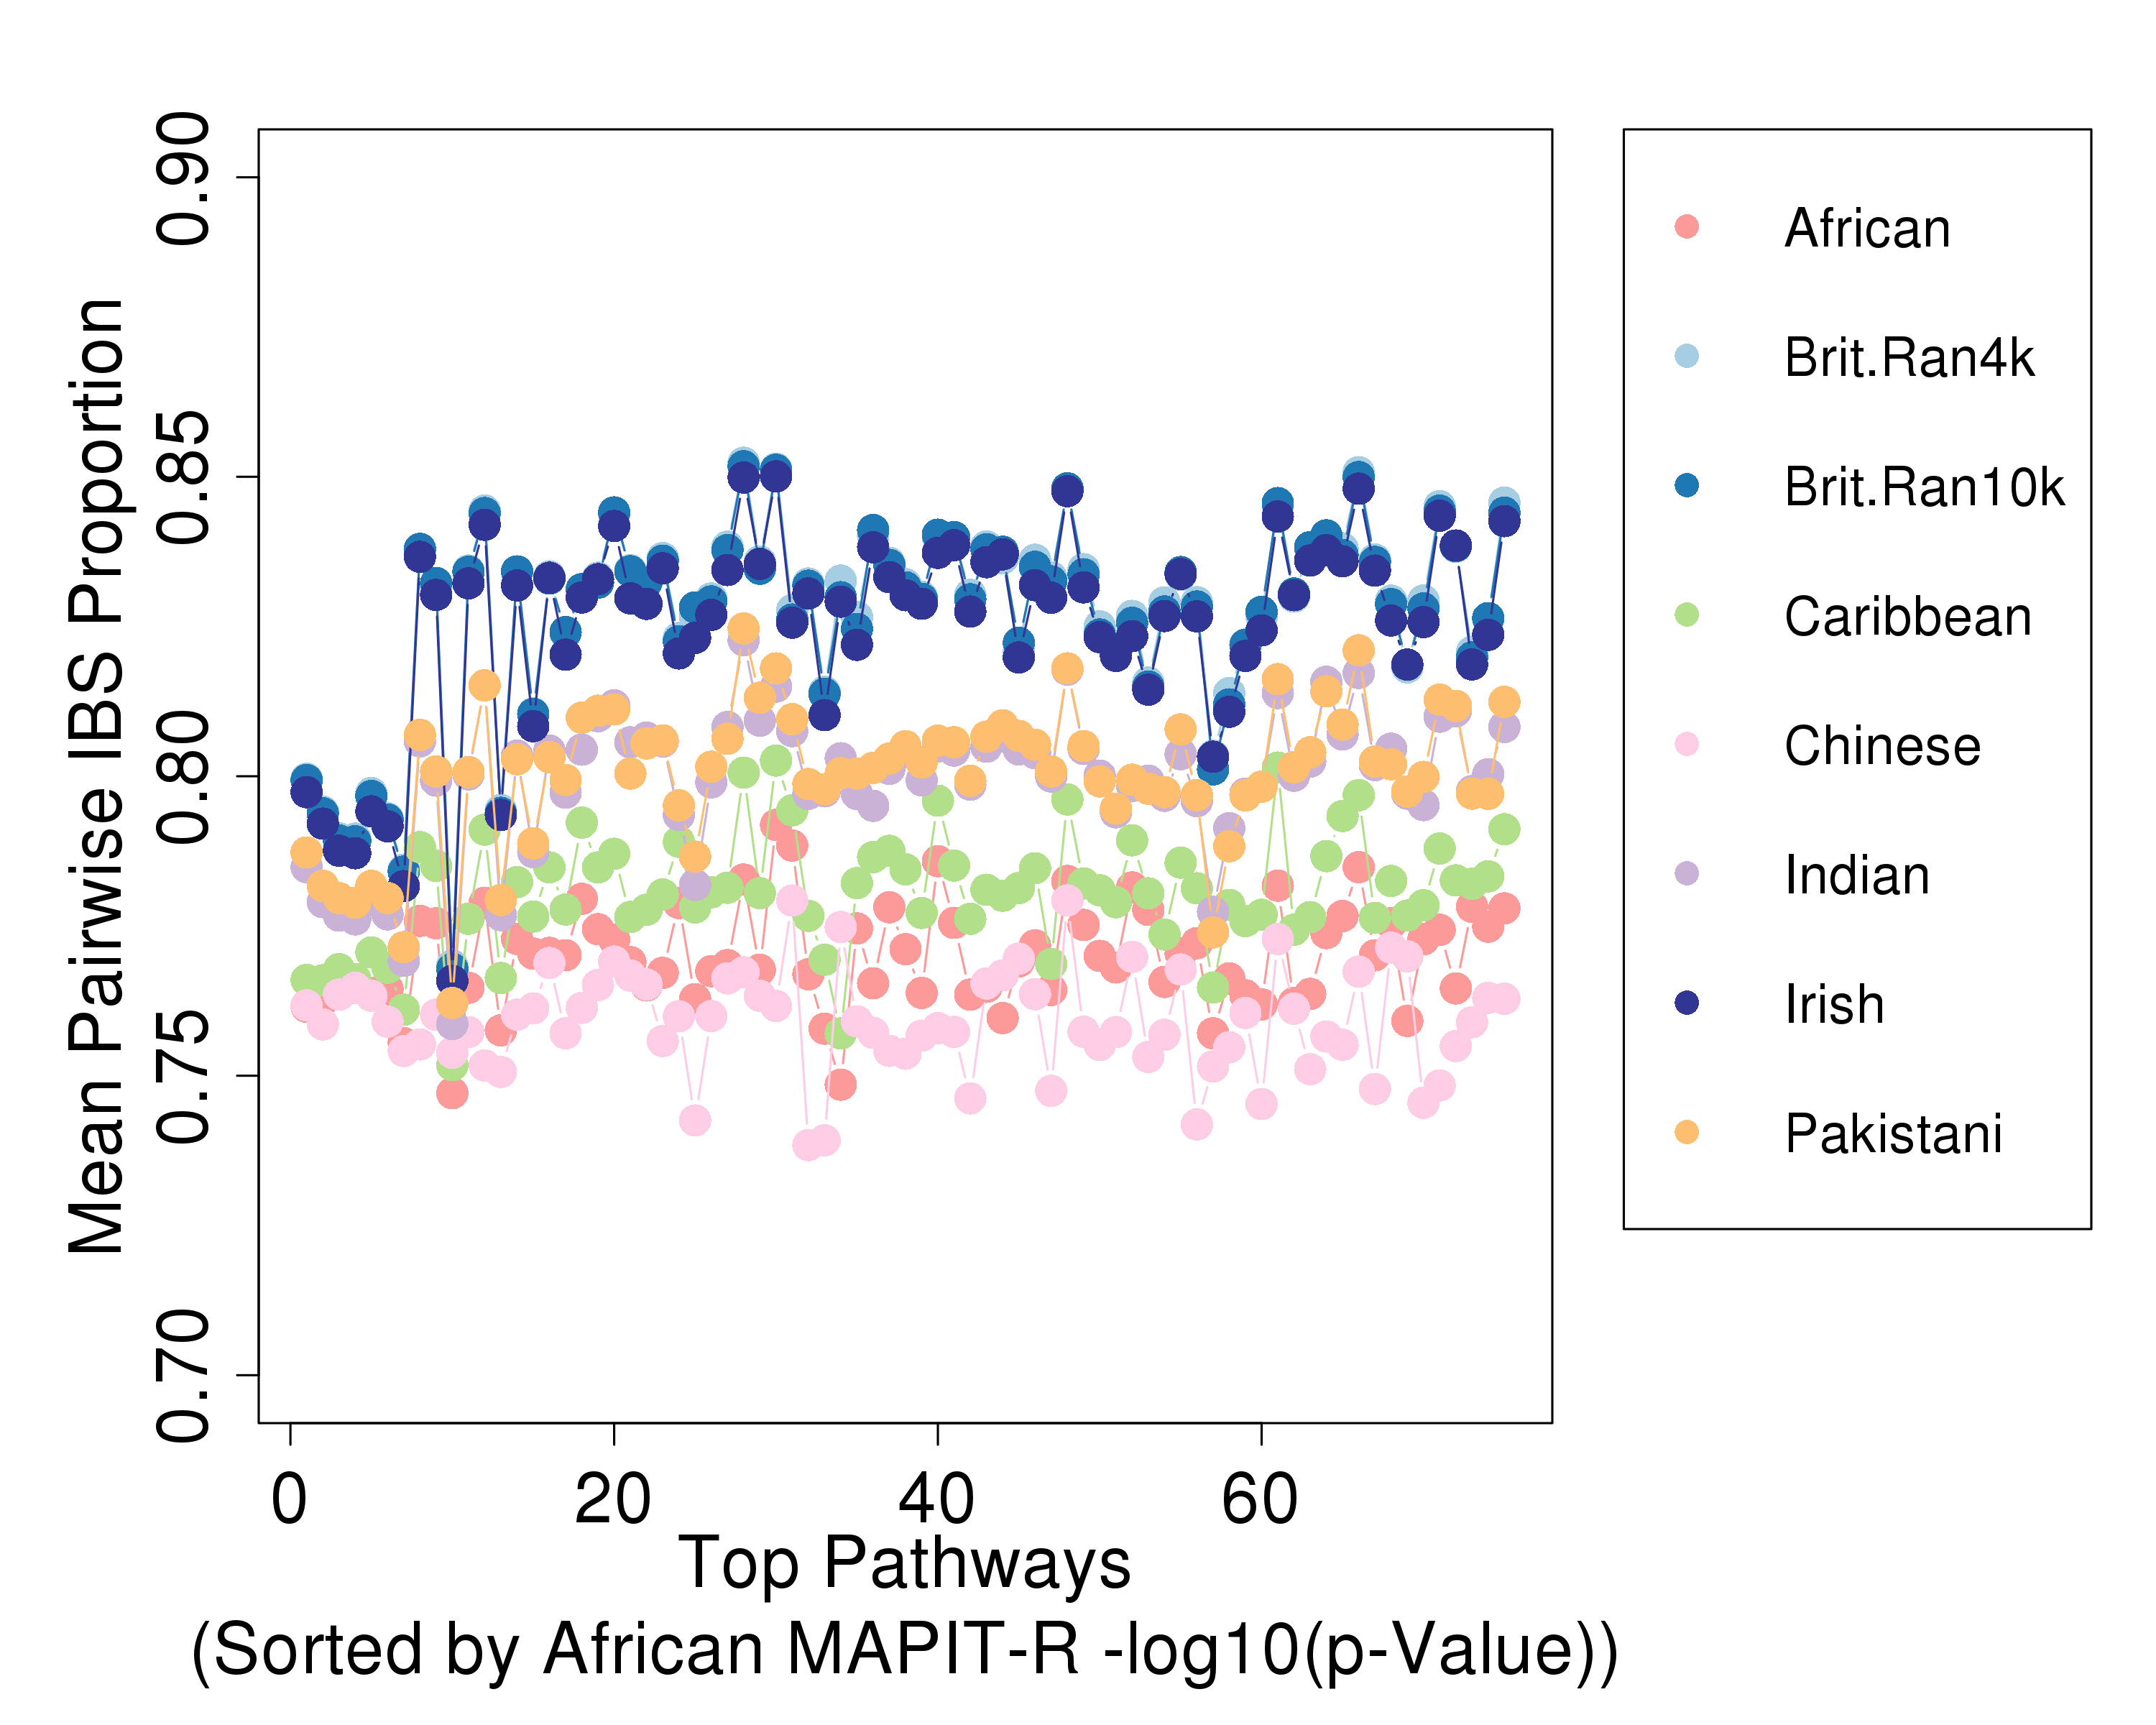
\includegraphics[scale=.35]{Images/Main/InterPath_Main_Figure_IBS_AllPopComps_vs2_AfrHght.png}
\caption[TBD]{\textbf{IBS in Top Pathways Across Populations}.}
\label{InterPath-Main-Figure-IBS-AllPopComps-AfrHght}
\end{figure}

\section{Discussion}\label{InterPath-Discussion}


\section{Online Methods}\label{InterPath-Online-Methods}

\subsection{UK BioBank Data}

\subsubsection{Population Subsets}
UK BioBank data was applied for and downloaded from XXX. We first grouped and extracted our multiple population subsets by using self-identified ancestry (`African', `British', `Caribbean', `Chinese', `Indian', `Irish', and `Pakistani'). British random subsets of 4,000 and 10,000 individuals, both the original sets and the additional four rounds of replications, were constructed by randomly choosing initial sets of non-overlapping 4,000 and 10,000 individuals; each round of 4,000 and 10,000 individuals were ensured not to overlap with the previous rounds of the same size of subset. Standard quality control (QC) procedures were employed on each population subset (see Supplementary Note for details). Note that unless stated otherwise, the genetic data used in these analyses were the directly genotyped variant sets from the UKB post-imputation on the University of Michigan Imputation Server \citep{Das2016}; most of the analyses in this manuscript utilized genetic relatedness matrices (GRMs), and GRMs have a stringent requirement of zero genotype missingness. To minimize the loss of SNPs while meeting this threshold we chose to impute missing genotypes while still focusing on just the original set of genotyped variants.

\subsubsection{Phenotypes}

For all the analyses presented in here, height and BMI were our complex traits of interest. Each phenotype was adjusted for age, gender, and assessment center. Following previous pipelines (cite GIANT), each dataset was first divided into male and female subsets. Age was then regressed out within each sex. The resulting residuals were then inverse normalized according to equation \#\# found in the supplement of (citation). These normalized values were then combined back between sexes, and, lastly, assessment center designations \textcolor{red}{(give UKB identifier?)} as detailed by the UKB were regressed out as well. 

\subsubsection{Global Principal Components}

To take into account possible global patterns of population structure, principal components to be used as covariates during analyses were derived by running PCA on our full set of UKB populations. FlashPCA2 was used to run PCA, and as stated, all of our post-QC, post-imputation population files were analyzed together.    

\subsection{GEMMA Analyses}

 the following variance component model:
\begin{equation}\label{InterPath-GEMMA-Equation-Model}
 \textbf{y} = \textbf{G}_1 + \textbf{G}_2 + \boldsymbol{\epsilon}
\end{equation}
where $y$ is a $n \times 1$ vector of phenotypes, $G_1$ is a $n \times n$ genetic relatedness matrix (GRM), constructed using all SNPs genome-wide and representing all first-order interactions, $G_2$ is a $n \times n$ matrix produced from the Hadamard product of $G_1$ against itself ($G_2 = G_1 \circ G_1$), representing all second-order interactions, and $\epsilon$ is a $n \times 1$ vector of normally distributed random effects. In other words, $G_1$ can be thought of as representing all additive effects, and $G_2$ can be thought of as representing all pairwise epistatic effects. To fit this model and estimate $G_2$, we used GEMMA \citep{Zhou2012} and its REML AI algorithm for estimating variance components.

GEMMA/GridLMM analyses were conducted using...

\subsection{PLINK Analyses}

PLINK pairwise epistasis analyses were conducted using PLINK v1.90b4 \citep{Purcell2007}, the `\texttt{-{}-epistasis}' command, and phenotypes that had top 10 global PCs regressed out; PCs were regressed out directly from the phenotypes due to the `\texttt{-{}-epistasis}' function having no explicit form to incorporate covariates. Default values for the `\texttt{-{}-epi1}' and `\texttt{-{}-epi2}' options (0.0001 and 0.01, respectively) were kept. And the PLINK model is as follows:
\begin{equation}
\textbf{y} = \beta_0 + \textbf{x}_1\beta_1 + \textbf{x}_2\beta_2 + \textbf{x}_1*\textbf{x}_2\beta_3    
\end{equation}
where \textbf{y} is once again a $n \times 1$ vector of phenotypes, $\beta_0$ is the y-intercept, $\textbf{x}_1$ is a $n \times 1$ vector of genotypes for SNP 1, $\beta_1$ is the corresponding additive effect size for $\textbf{x}_1$, $\textbf{x}_2$ is a $n \times 1$ vector of genotypes for SNP 2, $\beta_2$ is the corresponding additive effect size for $\textbf{x}_2$, $\textbf{x}_1 * \textbf{x}_2$ is the multiplicative interaction between $\textbf{x}_1$ and $\textbf{x}_2$, and $\beta_3$ is the corresponding effect size for $\textbf{x}_1 * \textbf{x}_2$. Our variable of interest of course is $\beta_3$ and whether this value significantly deviates from 0.  

\subsection{MAPIT Analyses}

MAPIT analyses were conducted using the MAPIT software downloaded from \url{https://github.com/lorinanthony/MAPIT}. MAPIT was run using the phenotypes as previously described and top 10 global PCs as covariates. The 

\noindent `\texttt{MAPIT\_Davies\_Approx}' function was used due to its computational speed up and having large enough sample sizes to properly employ the Davies approximation. 

To test for SNP-level marginal epistasis, we use MAPIT \citep{Crawford2017}. For a full derivation of the MAPIT framework please see \citet{Crawford2017}, but in short MAPIT begins with the following setup:
\begin{equation}
\textbf{y} = \mu + \textbf{x}_k\beta_k + \sum_{l \neq k} \textbf{x}_l\beta_l + \sum_{l \neq k} (\textbf{x}_k \circ \textbf{x}_l)\alpha_l + \boldsymbol{\epsilon}, \quad \boldsymbol{\epsilon} \sim \mathcal{MVN}(\textbf{0}, \tau^{2}\textbf{I})  
\end{equation}

where \textbf{y} is still a $n \times 1$ vector of phenotypes, $\textbf{x}_k$ is a $n \times 1$ vector of genotypes for our SNP of interest $k$, $\beta_k$ is our additive effect size for SNP $k$, $\textbf{x}_l$ is a $n \times 1$ vector of genotypes for every SNP $l$ that is not SNP $k$, $\beta_l$ is our additive effect size for SNP $l$, $(\textbf{x}_k \circ \textbf{x}_l)$ is the Hadamard product between our two SNP genotype vectors, $\alpha_l$ is interaction effect size, $\boldsymbol{\epsilon}$ is a $n \times 1$ vector of random effects which follow a multivariate normal distribution with mean $\textbf{0}$ and covariance matrix equal to variance effect $\tau$ times the $n \times n$ identity matrix $\textbf{I}$. In this model our parameter of interest would be $\alpha_l$, whether there is any significant interaction between our SNP of interest $k$ and of the remaining SNPs in the genome. However, as one might expect, the number of parameters in this model far exceeds the number of samples (ie $p >> n$), therefore making the solution indeterminable. To overcome this, MAPIT moves this setup into a linear mixed model framework and make the problem a variance component one. To do this, we put normal random priors on each of our effect sizes ($\beta_k$, $\beta_l$, and $\alpha_l$), and redefine our model as follows:
\begin{align}
    & \textbf{y} = \mu + \textbf{x}_k\beta_k + \textbf{m}_k + \textbf{g}_k + \boldsymbol{\epsilon} \\
    \textbf{m}_k \sim \mathcal{MVN}(\textbf{0}, &\omega^{2}\textbf{K}_k) \quad \textbf{g}_k \sim \mathcal{MVN}(\textbf{0}, \sigma^{2}\textbf{G}_k) \quad \boldsymbol{\epsilon} \sim \mathcal{MVN}(\textbf{0}, \tau^{2}\textbf{I}) \nonumber 
\end{align}
where $\textbf{m}_k$ and $\textbf{g}_k$ are both random effects that follow multivariate normal distributions, $\omega$ and $\sigma$ are their respective variance components, $\textbf{K}_k = \textbf{X}_{-k}\textbf{X}^{\textbf{T}}_{-k}/(p-1)$, the genetic relatedness matrix (GRM) constructed from all SNPs available aside from SNP $k$, and $\textbf{G} = \textbf{D}_k\textbf{K}_k\textbf{D}_k$, a GRM based on pairwise interaction terms between the $k$\textsuperscript{th} variant and all other variants. Here, we denote $\textbf{D}_k =$ diag$(\textbf{x}_k)$ to be an $n \times n$ diagonal matrix with the genotype vector $\textbf{x}_k$ as its diagonal elements. Our parameter of interest here is $\sigma$ and whether it is significantly larger from 0; a significant deviation would represent there exist some subset of genetic interactions between $k$ and the rest of the genome.

\subsection{MAPIT-R Model}

We describe the framework for ``\underline{Inter}actions in \underline{Path}way'' (MAPIT-R) analysis in detail here. The key goal of this method is to identify crosstalk between signaling pathways in GWAS, without having to explicitly model all possible higher-order interactions. In general, consider a pathway which is defined by a set of SNPs found within the regulatory regions of genes in that pathway. We will denote these variants with the set of indices $\mathcal{R} = (r_1,\ldots,r_p)$. Begin by considering the following partitioned linear regression model,
\begin{equation}\label{LM}
\by = \mu\bm{1}+\sum_{r\in \mathcal{R}}\bx_r\beta_{r}+\sum_{s\not\in \mathcal{R}}\bx_s\beta_{s}+\bvarepsilon, \quad \bvarepsilon\sim \mathcal{N}(\mathbf{0}, \tau^2\bI),
\end{equation}
where $\by$ is an $n$-dimensional vector of quantitative phenotypes for $n$ individuals; $\mu$ is an intercept term with an $n$-dimensional vector of ones; $\bx_r$ and $\bx_s$ are $n$-dimensional genotype vectors for variants that lie within and outside the regulatory region $\mathcal{R}$, respectively; $\beta_r$ and $\beta_s$ are the corresponding additive effect sizes; $\bvarepsilon$ is an $n$-vector of residual errors; $\tau^2$ is the residual error variance; $\bI$ denotes the identity matrix; and $\mathcal{N}(\bullet,\bullet)$ denotes a multivariate normal distribution. Here, we also assume that the genotypic vectors have been centered and standardized to have mean 0 and standard deviation 1.

Because we consider scenarios where there are more variants than samples, we need to specify additional modeling assumptions in Equation \eq{LM} to make the rest of the model identifiable. In particular, we recall previous approaches and assume that the individual effect sizes follow univariate normal distributions, or $\beta_r \sim \mathcal{N}(0, \omega^2/p)$ and $\beta_s \sim \mathcal{N}(0, \sigma^2/(l-p))$, where $l$ is the number of total number of all SNPs \citep{Crawford2017}. With the assumption of normally distributed effect sizes, the model defined in Equation \eq{LM} is equivalent to a variance component model where $\bg\sim \mathcal{N}(\bm{0}, \omega^2\bK)$ with $\bK=\bX_{\mathcal{R}}\bX_{\mathcal{R}}^{\T}/p$ being the genetic relatedness matrix computed using genotypes from all variants within the signaling pathway of interest; and $\wt\bg\sim \mathcal{N}(\bm{0}, \nu^2\wt\bK)$ with $\wt\bK=\bX_{-\mathcal{R}}\bX_{-\mathcal{R}}^{\T}/(l-p)$ representing a relatedness matrix computed using all other variants. Note that $\bg$ may be interpreted as a pathway's additive effect, while $\wt\bg$ denotes its polygenic background. 

To complete the specification of the MAPIT-R methodology, we lastly assume an additional random effect $\bu$ which models the summation of all pairwise interaction effects between a given signaling pathway variant and all other pathways. In this work, we limit ourselves to the case of finding second order crosstalk relationships between pathways --- although, extensions to higher-order interactions is straightforward \citep{Crawford2017}. Altogether, this results in the following linear mixed model
\begin{equation}
\by = \mu\bm{1}+ \bg +\wt\bg+\bu+\bvarepsilon,\\ 
\bg\sim \mathcal{N}(\bm{0}, \omega^2\bK), \quad \wt\bg\sim \mathcal{N}(\bm{0},
\nu^2\wt\bK),\\ 
\bu\sim\mathcal{N}(\bm{0},\sigma^2\bQ), \quad \bvarepsilon\sim \mathcal{N}(\mathbf{0}, \tau^2\bI).\label{LMM}
\end{equation}
Here, the $\bQ = \bK\circ\wt\bK$ is represents a second-order interaction relationship matrix, and is obtained by using the Hadamard product (i.e.~the squaring of each element) between the pathway specific relatedness matrix and its corresponding polygenic background. Note that the formulation of MAPIT-R in Equation \eq{LMM} can easily be extended to accommodate other fixed effects (e.g.~age, sex, or genotype principal components), as well as other random effects terms that can be used to account for sample non-independence due to other genetic or common environmental factors.

%Note that we make the assumption that each $\bg_k^{(l)}\sim \mbox{MVN}(\bm{0}, \sigma_{l}^2\bK^l_k)$, where the baseline covariance matrix $\bK_k=\bX_{-\mathcal{R}}\bX_{-\mathcal{R}}^{\T}/p_k$ is the conventional genetic relatedness matrix computed using genotypes from all $p_k$ variants outside of the region $\mathcal{R}$. Here, we use the power factor $l$ to denote the order of interaction (epistatic) effects that are accounted for within the model. For example, when $l=2$, $\mathbf{K}_k^2 = \mathbf{K}_k\circ\mathbf{K}_k$ represents a pairwise interaction relationship matrix, and is obtained by using the Hadamard product (i.e.~the squaring of each element) of the linear kernel matrix with itself \citep{Henderson:1985aa,Ronnegard:2008aa,Jiang:2015aa}. In this case, $\mathbf{K}_k^2$ denotes the marginal second order epistatic effect of the $k$\textsuperscript{th} functional marker under the polygenic background of all other markers. It is important to note that each $\bK_k^{l}$ changes with every new gene, protein, or pathway $k$ that is considered.

\subsection{Hypothesis Testing for Interaction Effects}

Our goal is to identify signaling pathways that have significant non-zero interaction effects on a given phenotype. To do so, we examine each $r$-th pathway of interest in turn, and test the null hypothesis in Equation \eqref{LMM} that $\text{H}_0: \sigma^2=0$. The variance component $\sigma^2$ effectively captures the total interaction effects between the $r$-th pathway and all other pathways. We refer to this as the marginal interaction effect for the $r$-th pathway. To do so, we make use of the MQS method for parameter estimation and hypothesis testing \citep{Zhou2017}. Briefly, MQS is based on the computationally efficient method of moments and produces estimates that are mathematically identical to the Haseman-Elston (HE) cross-product regression \citep{Haseman1972}. To estimate the variance components with MQS, we first multiply Equation \eq{LMM} by a projection (hat) matrix onto the null space of the intercept term $\mu$, where $\bH=\bI-\bm{1}(\bm{1}^{\T}\bm{1})^{-1}\bm{1}^{\T}$. After this projection procedure, we obtain a simplified linear mixed model 
\begin{equation}
\by^*_r = \bg^*_r +\wt\bg^*_r+\bu^*_r+\bvarepsilon^*_r\\ 
\bg_r\sim \mathcal{N}(\bm{0}, \omega^2\bK^*_r), \quad \wt\bg_r\sim \mathcal{N}(\bm{0}, \nu^2\wt\bK^*_r),\\ \bu_r\sim\mathcal{N}(\bm{0},\sigma^2\bQ^*_r), \quad \bvarepsilon_r\sim \mathcal{N}(\mathbf{0}, \tau^2\bH) \label{LMM2}
\end{equation}
where $\by^*_r=\bH\by$; $\bg^*_r = \bH\bg_r$; $\bK^*_r = \bH\bK_r\bH$; $\wt\bg_r^* = \bH\wt\bg_r$; $\wt\bK_r^* = \bH\wt\bK_r\bH$; $\bu^*_r = \bH\bu_r$; $\bQ^*_r = \bH\bQ_r\bH$; and $\bvarepsilon_r^* = \bH_r\bvarepsilon$, respectively. Then for each pathway considered, the MQS estimate for the marginal interaction effect is computed as
\begin{equation}
\wh\sigma^2 = \by^{*\T}_r\bA_r\by
\end{equation}
where $\bA_{r} = (\bS_r^{-1})_{31}\bK_r^*+(\bS_r^{-1})_{32}\wt\bK_r^*+(\bS_r^{-1})_{33}\bQ^*_r+(\bS_r^{-1})_{34}\bH$ with elements $(\bS_r)_{jk} = \tr(\bSigma_{rj} \bSigma_{rk})$ for the covariances matrices subscripted as $[\bSigma_{r1}; \bSigma_{r2}; \bSigma_{r3}; \bSigma_{r4}]  = [\bK^*_r; \wt\bK^*_r; \bQ^*_r; \bH]$. Here, $\tr(\bullet)$ is used to denote the matrix trace function. It has been shown that, under MQS, a given marginal variance component estimate $\wh\sigma^2$ follows a mixture of chi-square distributions under the null hypothesis \citep{Crawford2017}. Namely, $\wh\sigma^2 \sim \sum_{i=1}^{n}\lambda_{i}\chi^2_{1,i}$, where $\chi^2_{1}$ are chi-square random variables with one degree of freedom and $(\lambda_{1},\ldots,\lambda_{n})$ are the eigenvalues of the matrix 
\begin{equation*}
\left(\wh\omega^2_{0}\bK^*_r+\wh\nu^2_{0}\wt\bK^*_r+\wh\tau^2_{0}\bH\right)^{1/2} \bA_{r}\left(\wh\omega^2_{0}\bK^*_r+\wh\nu^2_{0}\wt\bK^*_r+\wh\tau^2_{0}\bH\right)^{1/2}
\end{equation*}
with $(\wh\omega^2_{0},\wh\nu^2_{0},\wh\tau^2_{0})$ being the MQS estimates of $(\omega^2,\nu^2,\tau^2)$ under the null hypothesis. Several approximation and exact methods have been suggested to obtain p-values under the distribution of $\wh\sigma^2$. One frequented choice is Davies exact method \citep{Davies1980,Wu2011}. 

%\subsection*{Hypothesis Testing for Overall Associations}

%FORCE also provides an option for summarizing overall marker enrichment. Here, we assume that we have already computed the $q$ marginal effect p-values for genetic marker $k$, denoted as $\wh\bp_k = (\wh p_{k1},\ldots,\wh p_{kq})$. Let $\wh\balpha_k^* = F^{-1}(\wh\bp_k)$ be the transformed test statistic where $F^{-1}$ is the inverse of the cumulative distribution function (CDF) of the standard chi-square $\chi^2_1$. We follow previous works and define the sum of the correlated chi-square variables for a given functional genomic marker as \citep{Nakka:2016aa}
%\begin{equation}
%\bar{\alpha}_k^* = \sum_{l=1}^{q}\wh\alpha_{k,l}^*.\label{Comp}
%\end{equation}
%(NOTE: Follow the rest of the language from methods in PEGASUS here).

\section{URLs}\label{InterPath-URLs}

MAPIT: \url{https://github.com/lorinanthony/MAPIT}
MAPIT-R: \url{https://github.com/mturchin20/MAPIT-R}

\section{Acknowledgments}\label{InterPath-Acknowledgments}

\section{Author Contributions}\label{InterPath-Author-Contributions}

\section{Competing Interests}\label{InterPath-Competing-Interests}

\nolinenumbers

\begingroup
\bibliographystyle{apalike}
\setstretch{1.0}
\bibliography{Main}
\endgroup









\iffalse

SCRAP

Information idea about creating random 'pathways' that have either the same number of genes or SNPs to show that it has to be the *right* collection of information/materials to get the same amount of significance

\subsubsection{Power Gained from Proper Pathway Definitions}

Running a GWAS of height and BMI on each of our population subsets with PLINK, we find only one genome-wide significant hit (Figure \ref{InterPath-Main-Figure-GWAS-Height} \& Supplementary Figure \ref{InterPath-Supp-Figure-GWAS-BMI}). And further similarly to before, we also find a handful of marginally significant variants. More interestingly however, we now ask how similar the MAPIT and GWAS results are. And indeed, comparing the two sets of genome-wide analyzes, we see a wide range of different genetic architecture patterns being represented (Figure \ref{InterPath-Main-Figure-MAPITvsGWAS-AfrHght} \& Supplementary Figure \ref{InterPath-Supp-Figure-MAPITvsGWAS}). Focusing on the African subset and height, we find 49 SNPs that are only marginally significant in MAPIT, 50 SNPs that are only marginally significant in the GWAS, and 0 SNPs that are marginally significant in both tests. Despite the lack of power to identify genome-wide significant results, we still see a strong representation of the partition of additive and epistatic effects in our results. 

\begin{figure}[htbp]
\centering
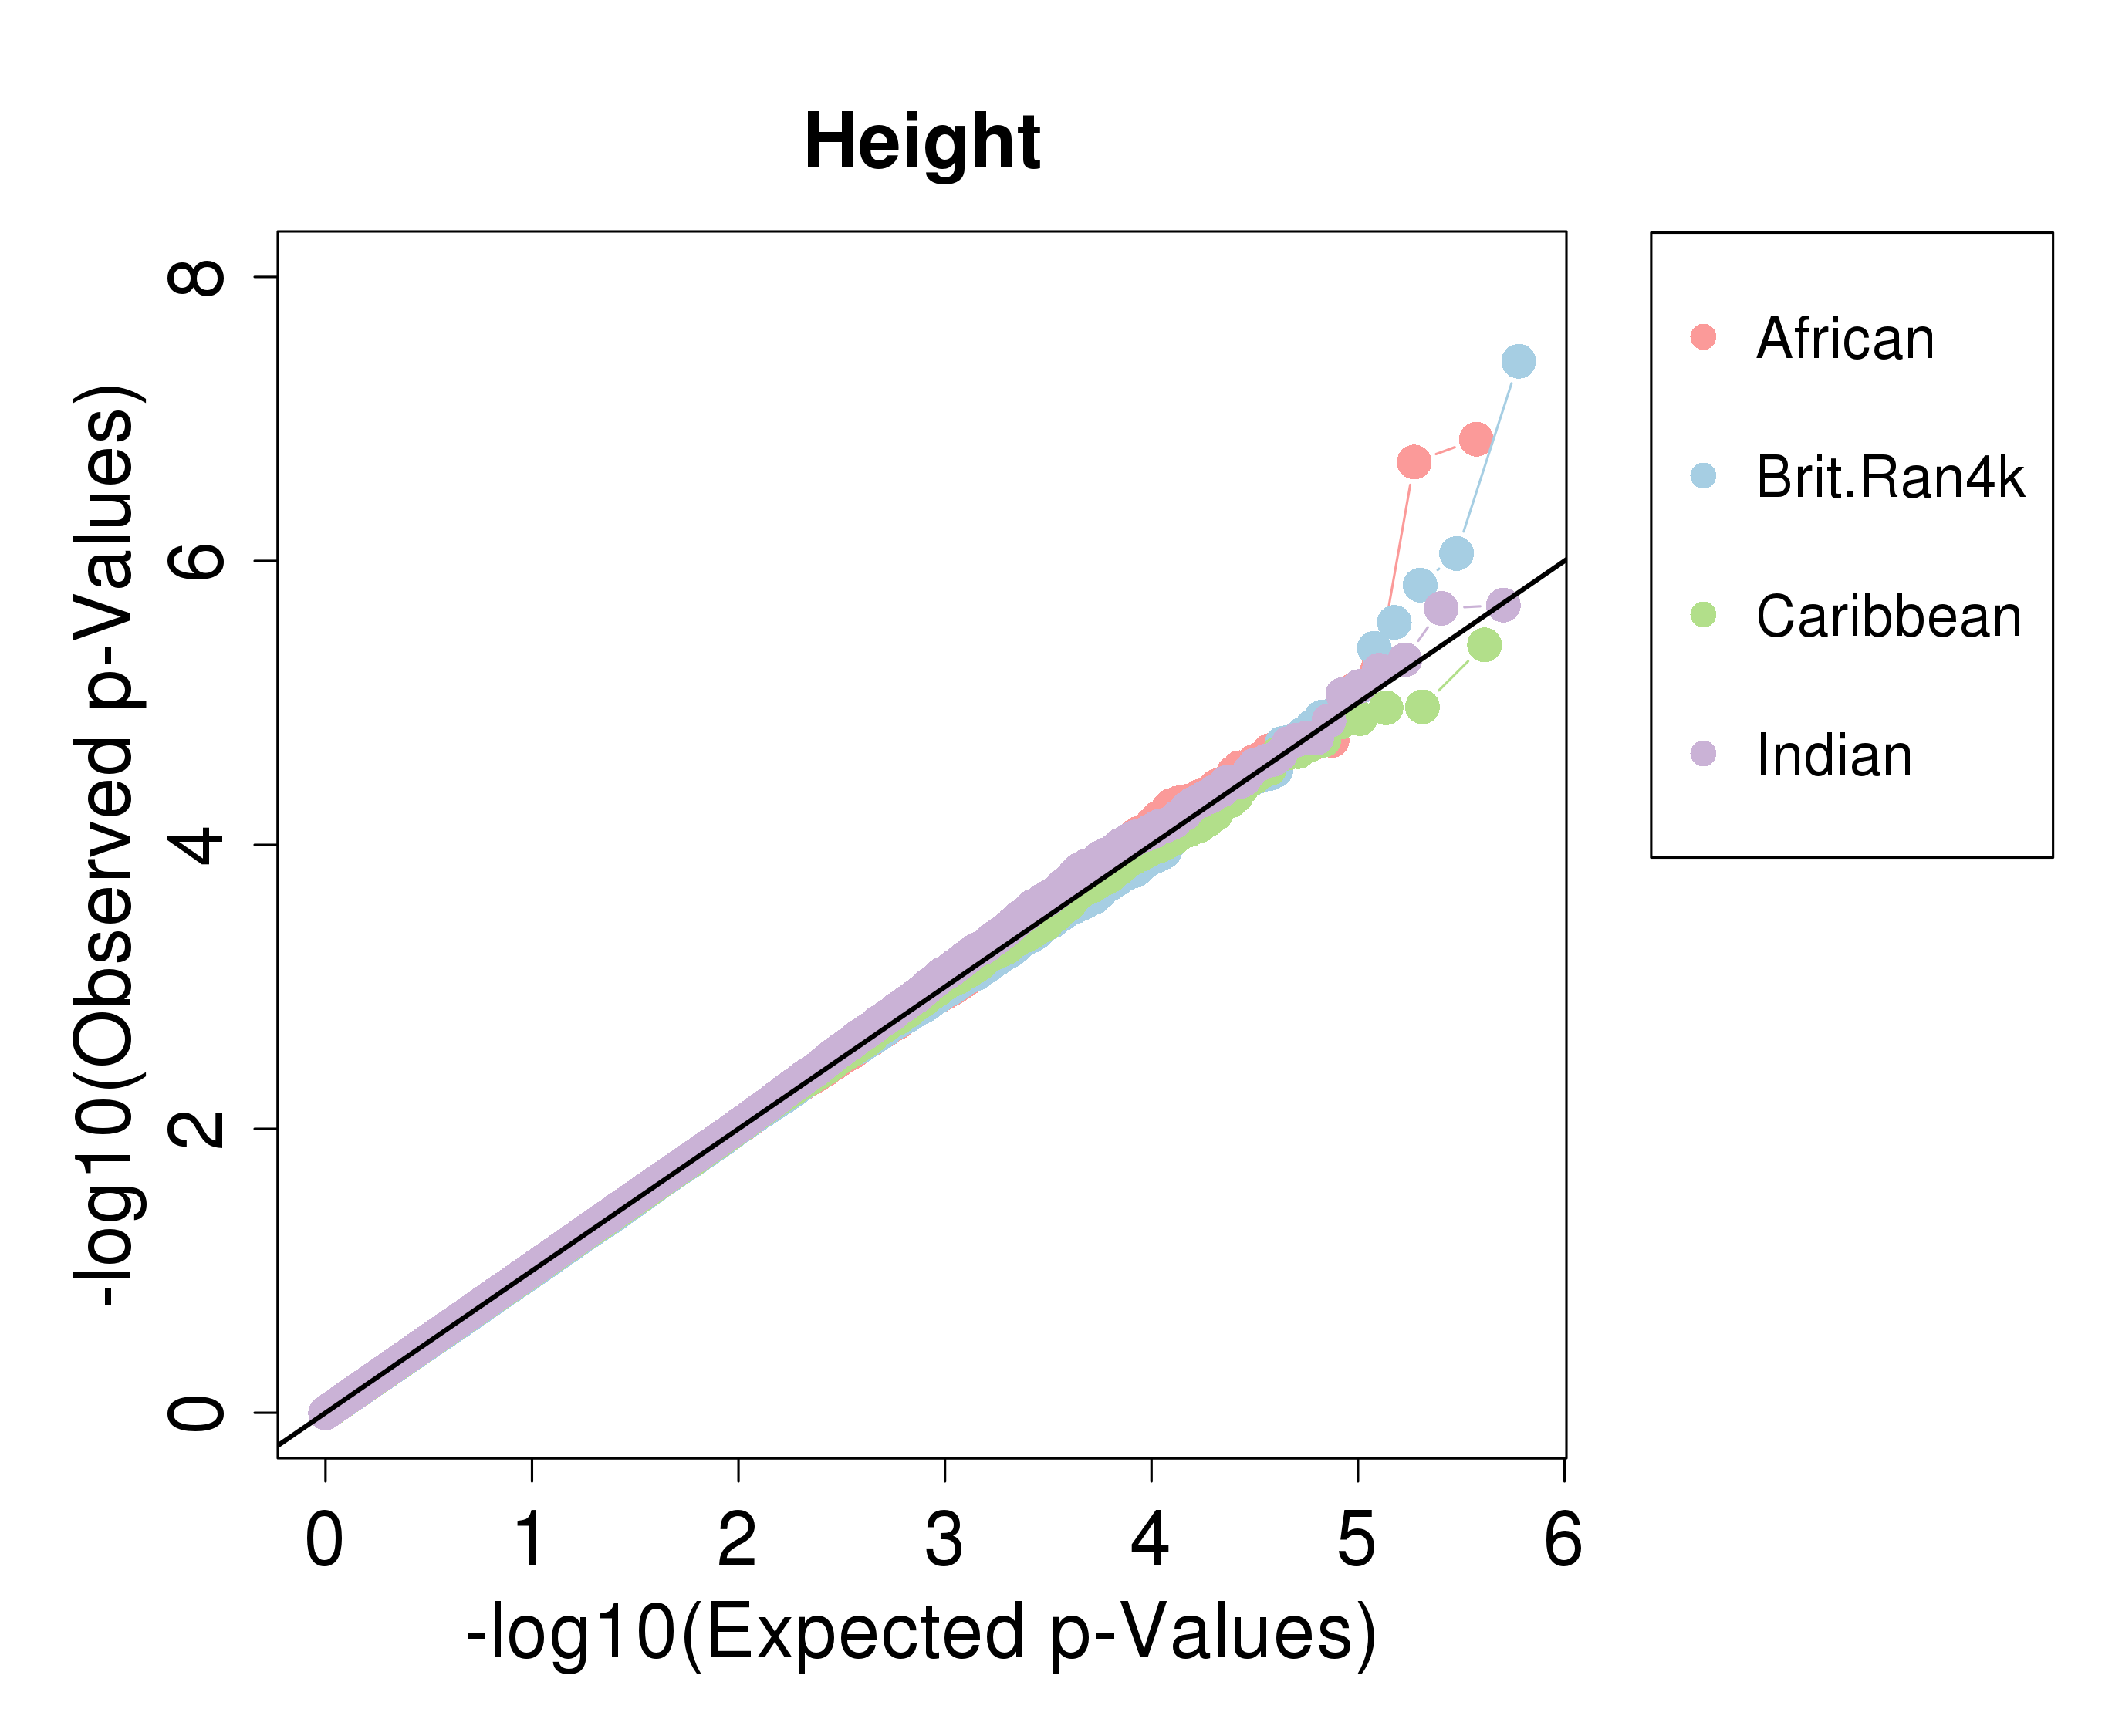
\includegraphics[scale=.35]{Images/Main/InterPath_Main_Figure_GWAS_vs2_Height.png}
\caption[TBD]{\textbf{GWAS Results QQ-Plots}.}
\label{InterPath-Main-Figure-GWAS-Height}
\end{figure}

\begin{figure}[htbp]
\centering
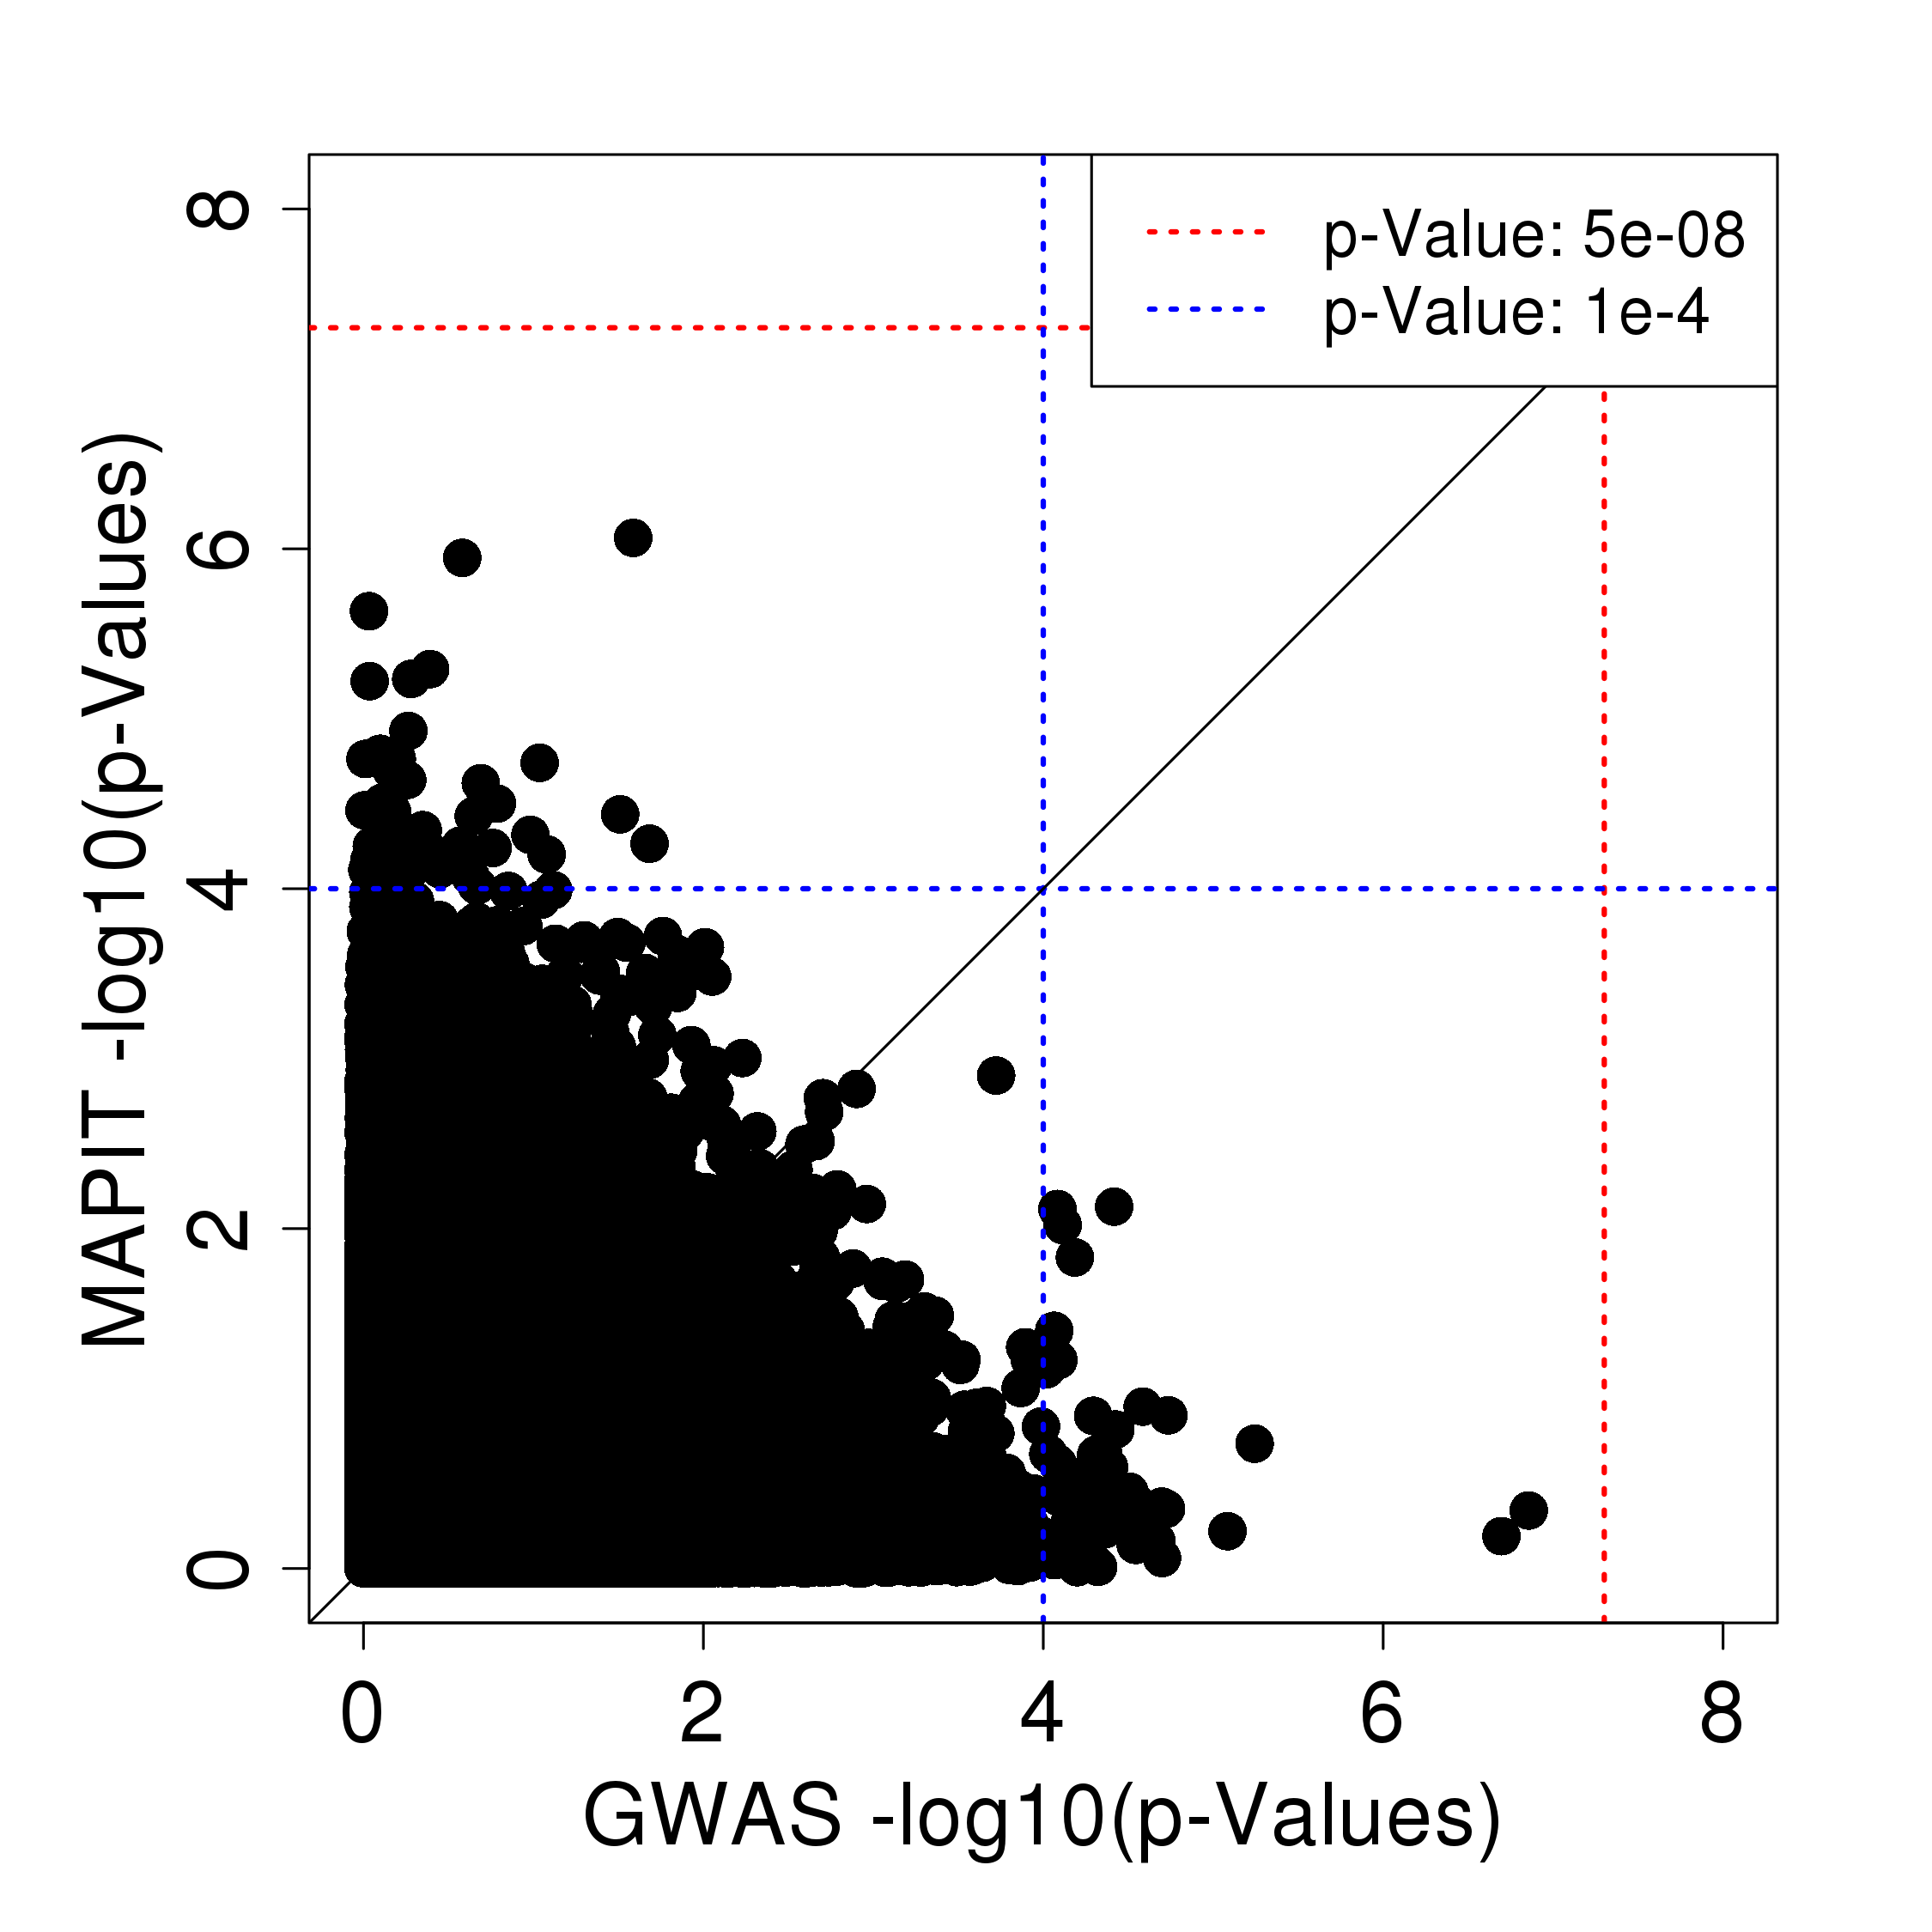
\includegraphics[scale=.35]{Images/Main/InterPath_Main_Figure_MAPITvsGWAS_vs2_AfrHght.png}
\caption[TBD]{\textbf{MAPIT vs. GWAS Results}.}
\label{InterPath-Main-Figure-MAPITvsGWAS-AfrHght}
\end{figure}

\textcolor{red}{(NOTE: below is what we were expecting for these results. But as you can see, the GIANT height/bmi results don't align in the way were anticipating. They are more spread out between height and BMI. I have checked though that the GIANT p-values of these top 500 SNPs are more correlated with our GWAS p-values than our MAPIT p-values (like ~.17 vs. .05). 
I think one alternative approach to this section is to angle instead as: 'we do not have power to even see a difference in GWAS vs. MAPIT as we were anticipating, thus indicating our real need to increase power. Hence, we moved forward with a method that we believed was going to accomplish that').}

To help further get a sense of whether these results are revealing patterns in true biology, we also annotated the top 500 SNPs with the most significant height and BMI GWAS $p$-values from the 2018 GIANT and UKB meta-analysis \cite{Yengo2018} in both our GWAS and MAPIT results. As expected, these 500 SNPs are heavily represented among the tail end of the most significant GWAS results, but maybe less expected is just how insignificant these SNPs appear on the MAPIT list of top results (\textcolor{red}{Supplementary Table -- listing differences in ranking of these 500 SNPs between GWAS and MAPIT}). In fact looking across the genome it is easy to see how different the relative ranking of SNPs are between the GWAS and MAPIT results (Figures \ref{InterPath-Main-Figure-MAPITvsGWAS-Manhattan}D \& \ref{InterPath-Main-Figure-MAPITvsGWAS-Manhattan}E). It is clear that even with our limited sample sizes, differences in the trends of importance of additive versus epistatic signals can be observed among marginally significant SNPs.  

\begin{figure}[htbp]
\centering
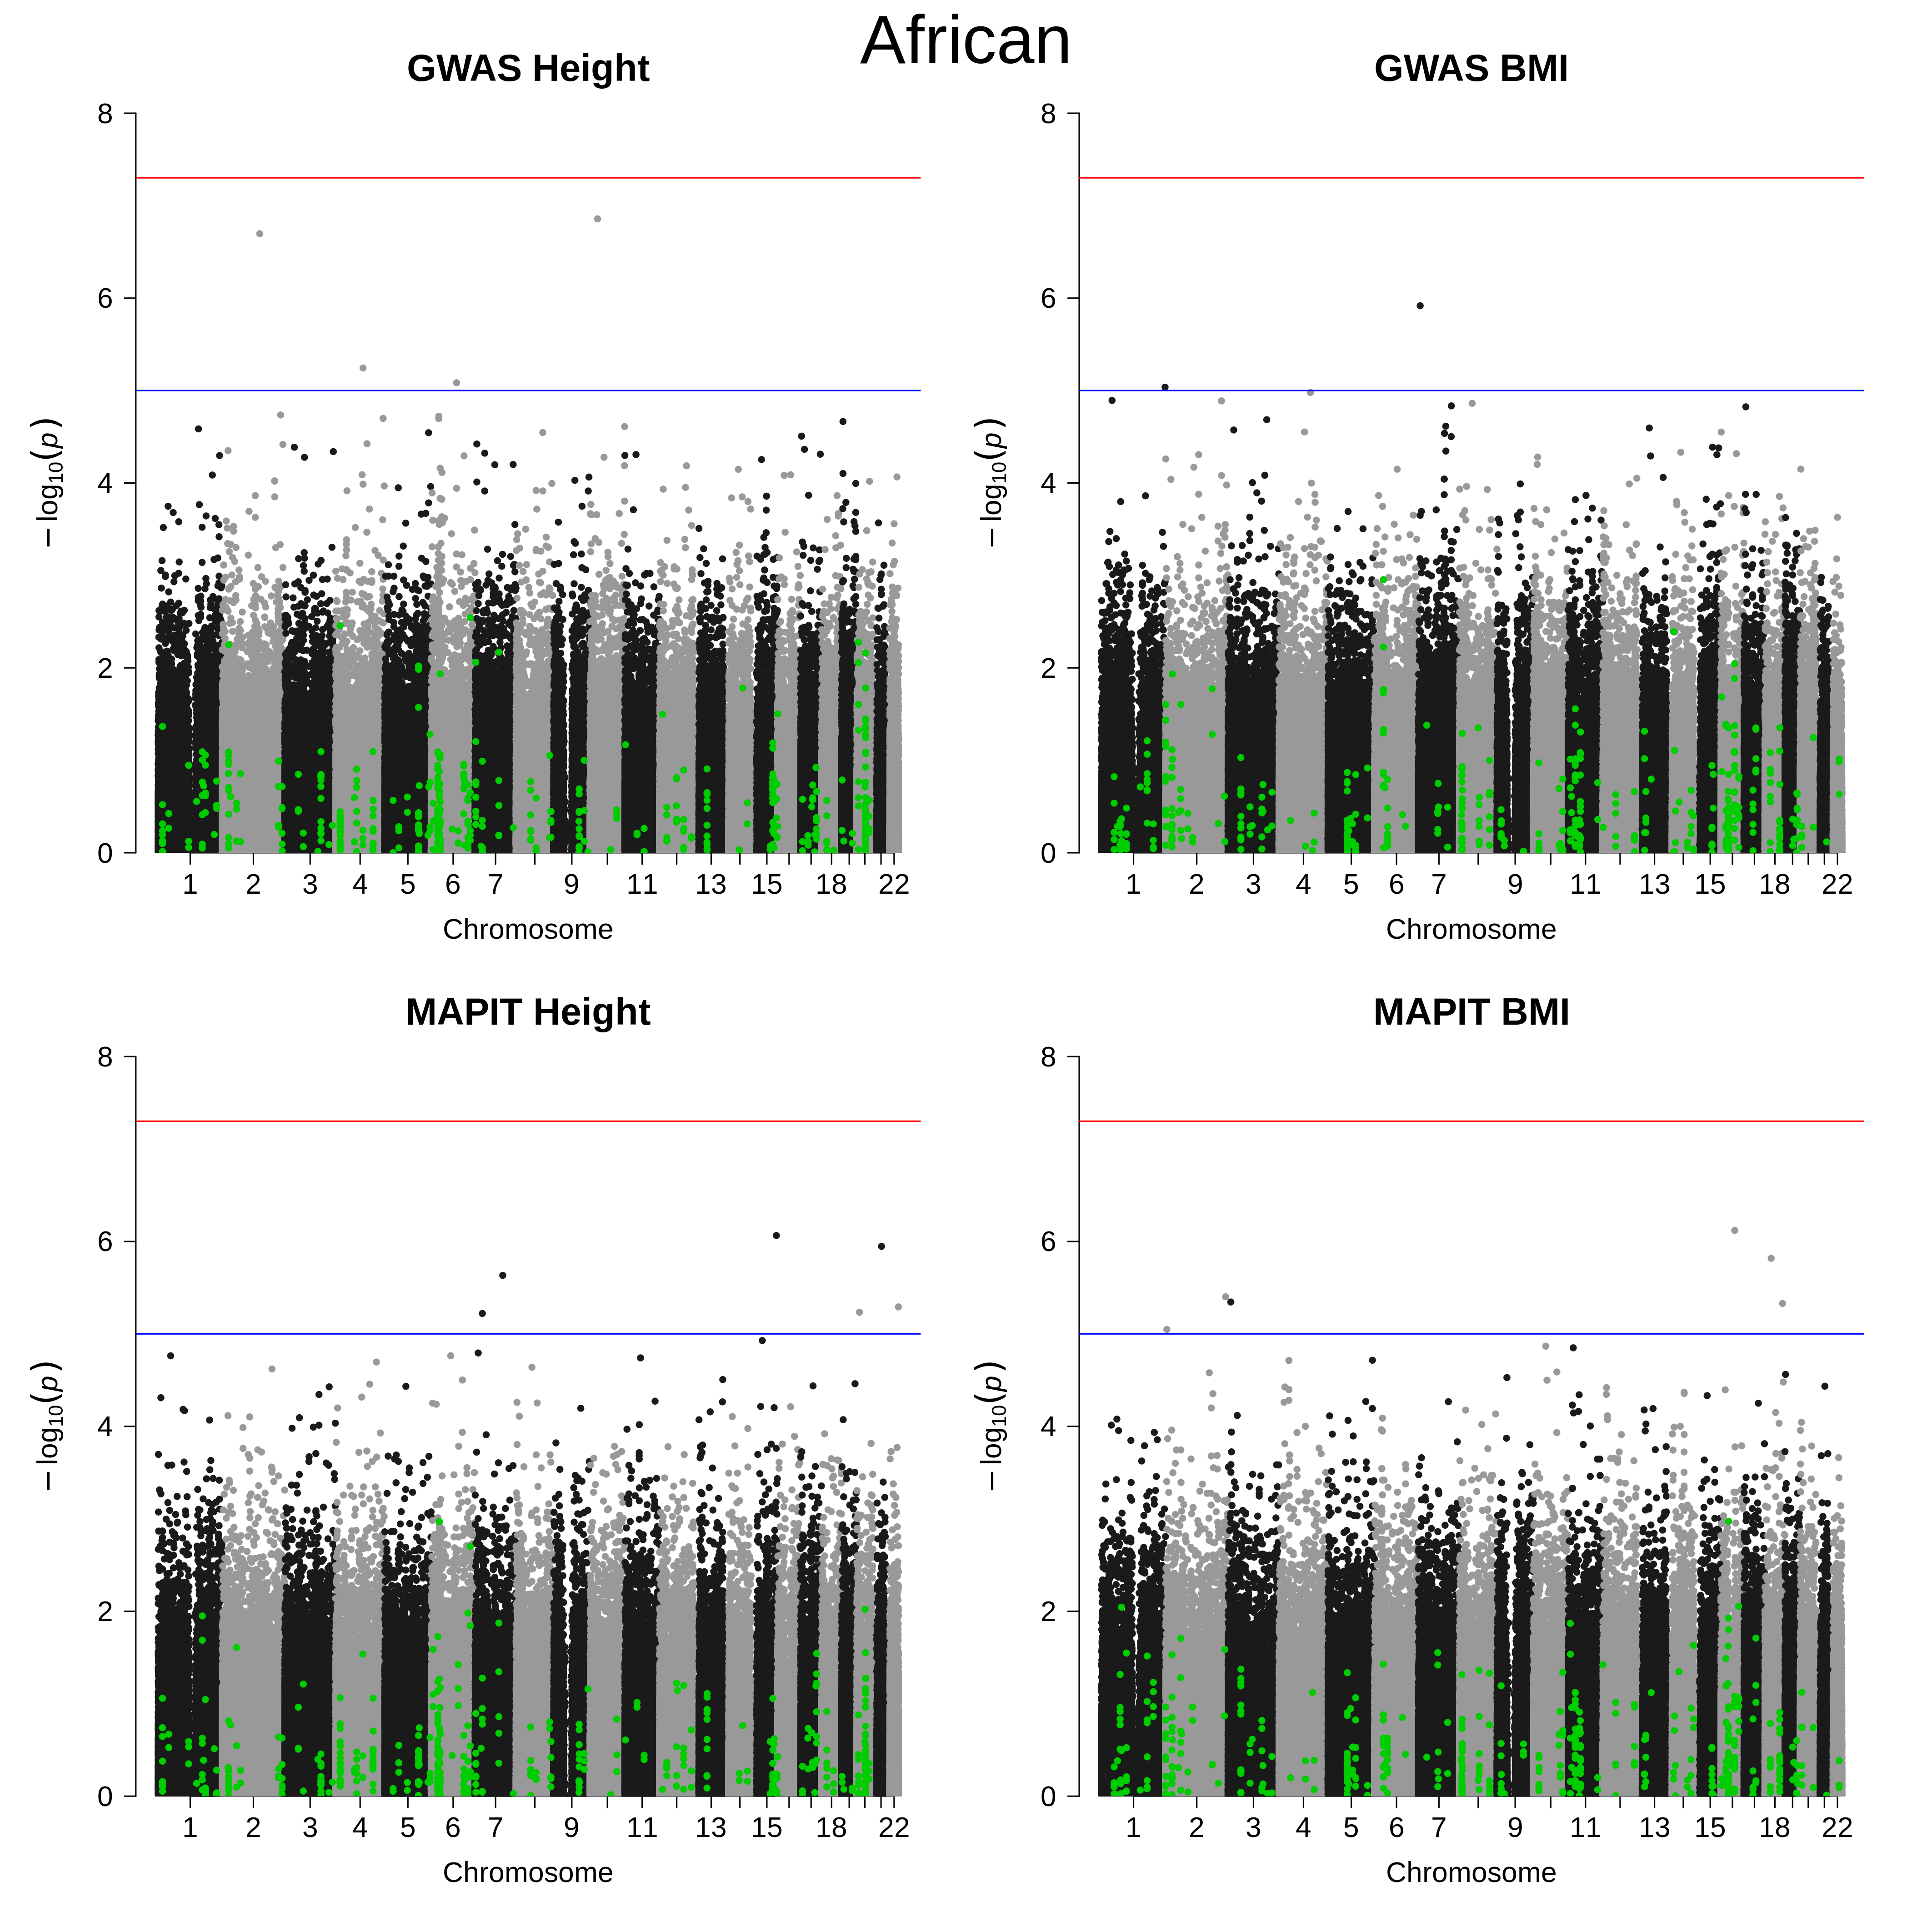
\includegraphics[scale=.35]{Images/Main/InterPath_Main_Figure_MAPITvsGWAS_Manhattan_vs1.png}
\caption[TBD]{\textbf{MAPIT \& GWAS Manhattan Plots}. \textcolor{red}{will be just height, MAPIT on top (D), GWAS on bottom (E), each plot wider. Green dots are the 500 SNPs that have the most significant GIANT/UKB p-values.}}
\label{InterPath-Main-Figure-MAPITvsGWAS-Manhattan}
\end{figure}

%\begin{figure}[htbp]
%\centering
%\includegraphics[scale=.35]{Images/Main/InterPath_Main_Figure_GWAS_Manhattan_vs1.png}
%\caption[TBD]{\textbf{GWAS Manhattan Plot}.}
%\label{InterPath-Main-Figure-GWAS-Manhattan}
%\end{figure}

\fi

\end{document}
